\section{Resultados}\label{sec:resultados}

Los resultados se presentan en el orden en que condicionaron las decisiones
siguientes: primero la estructura espacial que justifica un enfoque
territorial (§\ref{sec:res-espacial}); después la comparación de modelos de
conteo, que reveló que el error dominante es municipal
(§\ref{sec:res-conteo}); luego el ajuste del modelo jerárquico que se
construyó en respuesta (§\ref{sec:res-jerarquico}), y al final la validación
de todos contra 2024 (§\ref{sec:res-validacion}). Todas las cifras se refieren
a la partición de 2\,241 celdas hexagonales de 500\,m de lado descrita en
§\ref{sec:met-unidad}.

% ---------------------------------------------------------------------------
\subsection{Estructura espacial de la siniestralidad}\label{sec:res-espacial}
% ---------------------------------------------------------------------------

\paragraph{Concentración.}
Los accidentes de 2019--2024 se reparten de forma muy desigual entre las
celdas (figura~\ref{fig:res-conteos}): la mediana por celda es 30 y el máximo
3\,741. La curva de Lorenz da un \textbf{coeficiente de Gini de 0,766}. El
1\,\% de las celdas concentra el 14,9\,\% de los accidentes; el 5\,\%, el
43,7\,\%, y el 10\,\%, el 61,7\,\%. A escala de intersección el Gini es 0,752
y el 5\,\% de los puntos concentra el 58\,\% (figura~\ref{fig:res-lorenz}). La
concentración es prácticamente la misma en las dos escalas: es la firma de
una distribución de cola pesada y no un artefacto de la agregación.

\begin{figure}
\centering
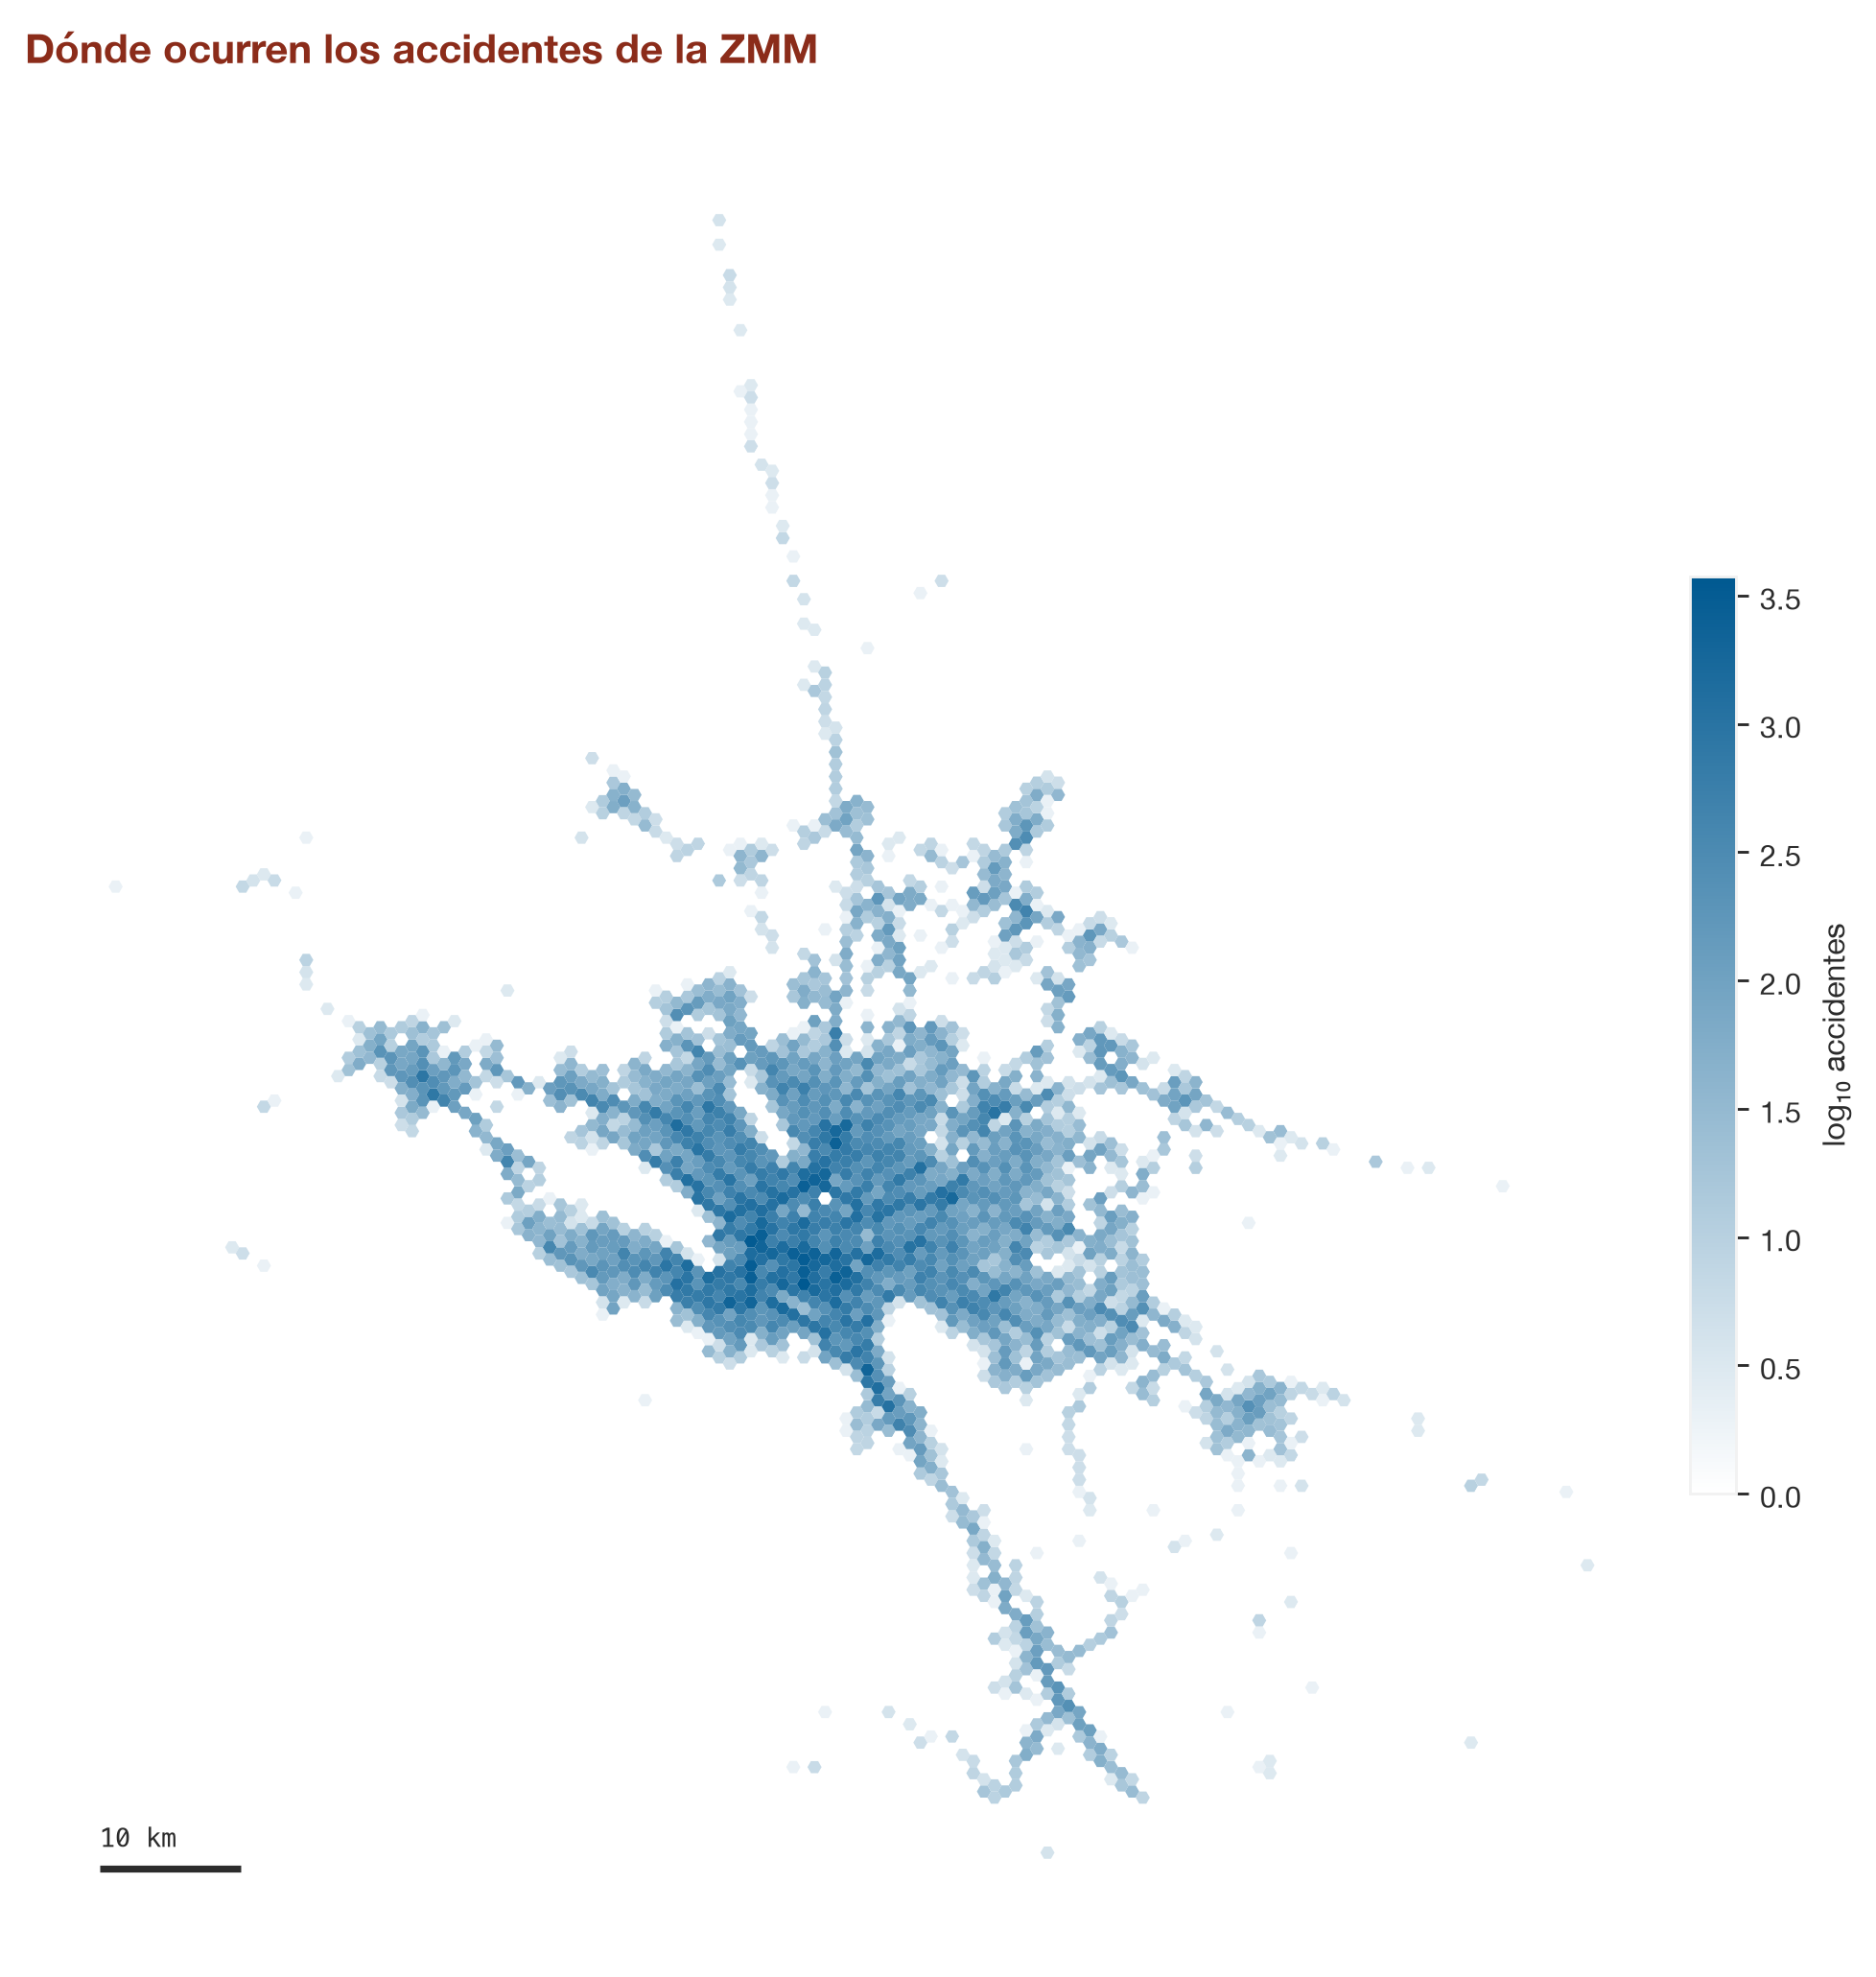
\includegraphics[width=\columnwidth]{conteos_hex}
\caption{Accidentes por celda hexagonal, 2019--2024, en escala
logarítmica. La mediana por celda es 30; el máximo, 3\,741.}
\label{fig:res-conteos}
\end{figure}

\begin{figure}
\centering
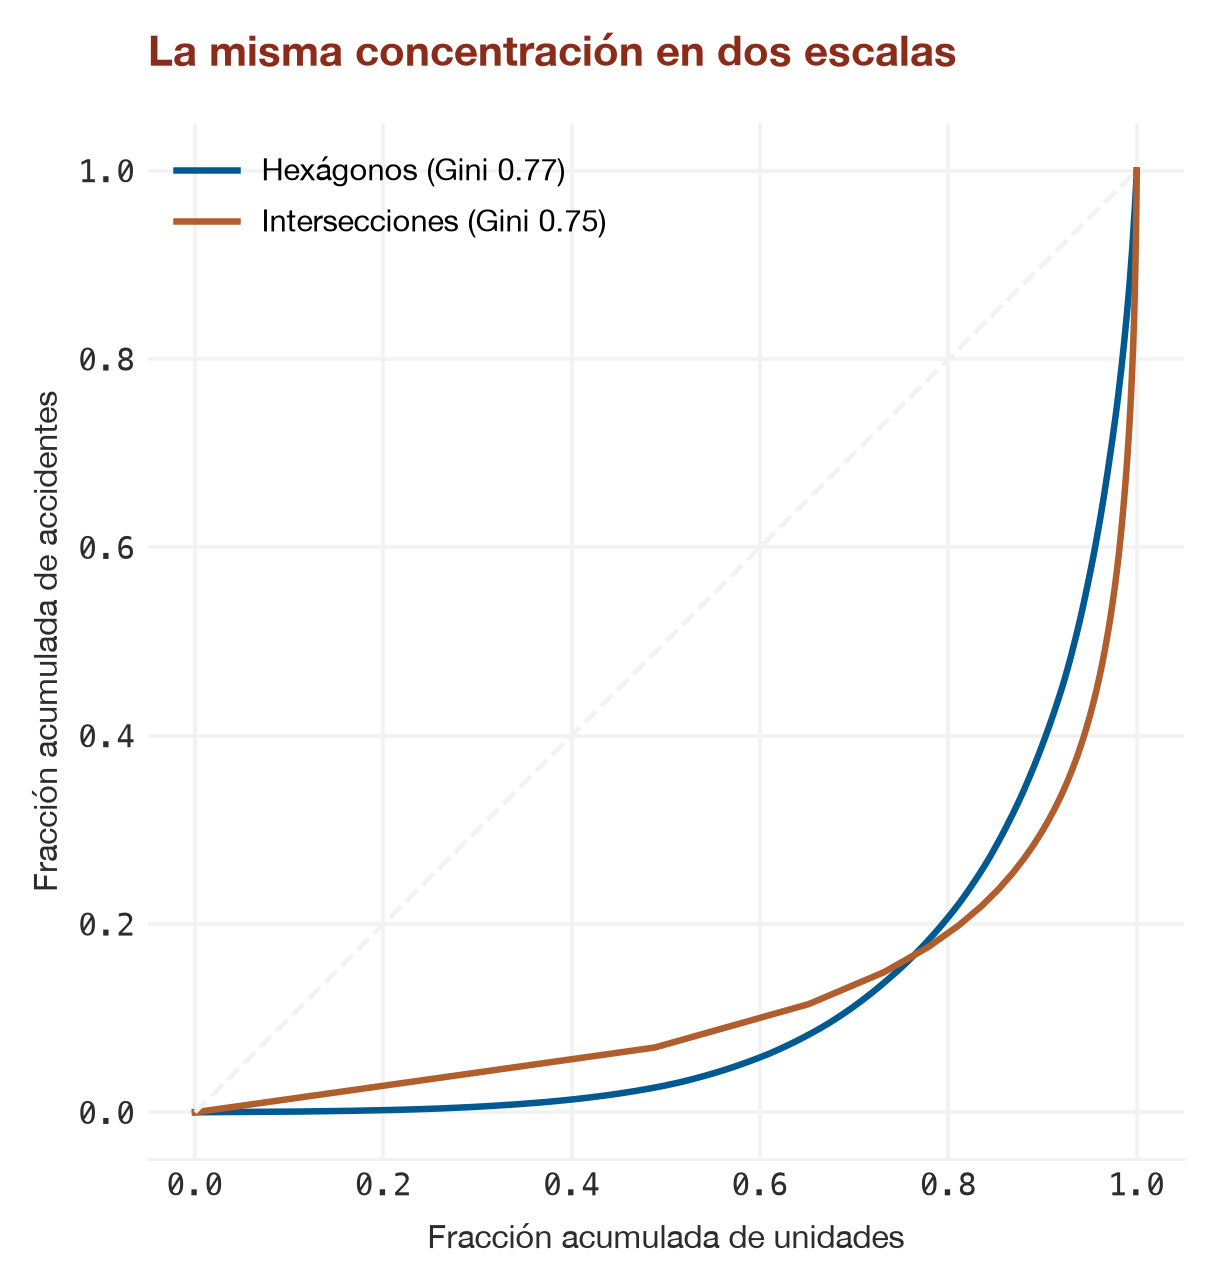
\includegraphics[width=0.85\columnwidth]{lorenz_escalas}
\caption{Curvas de Lorenz por celda hexagonal y por intersección. La
desigualdad es casi idéntica a ambas escalas (Gini 0,77 y 0,75).}
\label{fig:res-lorenz}
\end{figure}

\paragraph{Autocorrelación global.}
Con pesos de contigüidad estandarizados por fila sobre $\log(1+n)$, el
\textbf{$I$ de Moran es 0,648}, con $z = 37$ frente a 999 permutaciones
(figura~\ref{fig:res-moran}); ninguna permutación se acerca al valor
observado. Sobre el conteo crudo el estadístico es 0,57, de modo que la
conclusión no depende de la transformación. Las celdas vecinas se parecen:
un modelo que las trate como independientes subestimará sus errores
estándar.

\begin{figure*}
\centering
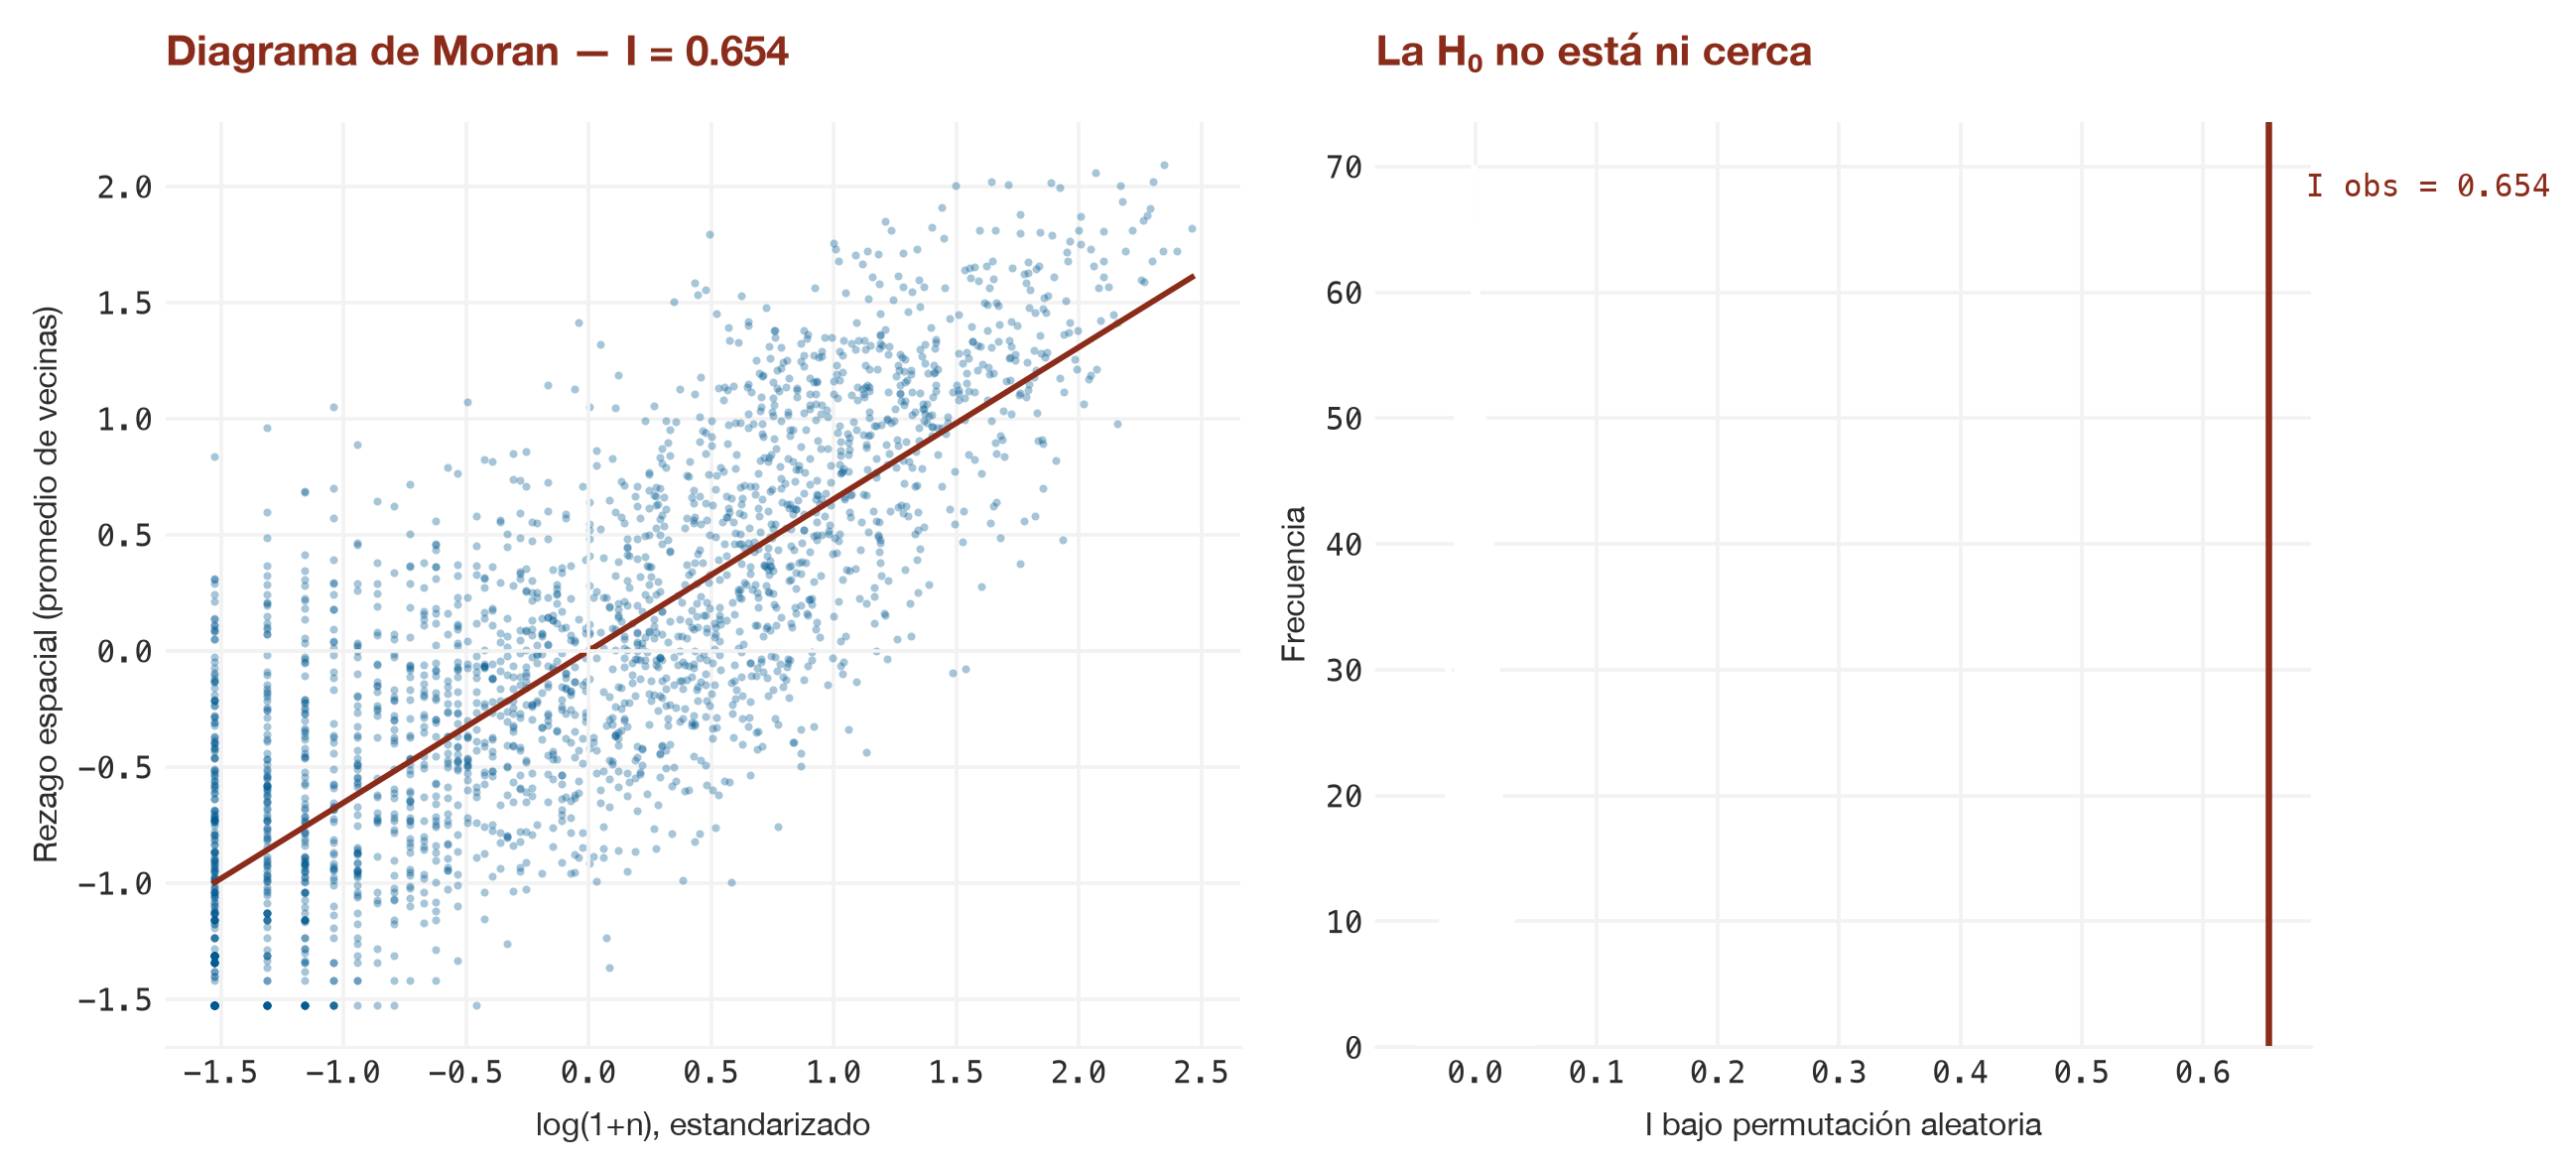
\includegraphics[width=0.85\textwidth]{moran}
\caption{Izquierda: diagrama de dispersión de Moran sobre $\log(1+n)$
estandarizado; la pendiente es $I = 0{,}648$. Derecha: distribución de $I$
bajo 999 permutaciones aleatorias, concentrada alrededor de cero, frente al
valor observado.}
\label{fig:res-moran}
\end{figure*}

\paragraph{Sensibilidad a la escala.}
Repetir el análisis con lados de 250 y 1\,000\,m
(cuadro~\ref{tab:res-maup}) muestra el efecto de escala esperado en el $I$ de
Moran, que crece con la agregación de 0,52 a 0,72, mientras que la
concentración apenas cambia (el 5\,\% superior concentra entre el 43 y el
45\,\% de los accidentes en las tres rejillas). La autocorrelación es una
propiedad del fenómeno y no de la rejilla elegida.

\begin{table}
\centering\small
\caption{Sensibilidad de la autocorrelación y la concentración al tamaño de
la celda.}
\label{tab:res-maup}
\begin{tabular}{@{}rrrrr@{}}
\toprule
Lado (m) & Celdas & $I$ & Gini & Top 5\,\% \\
\midrule
250     & 6\,145 & 0,524 & 0,746 & 44,8\,\% \\
500     & 2\,241 & 0,648 & 0,756 & 42,6\,\% \\
1\,000  &    815 & 0,721 & 0,788 & 43,5\,\% \\
\bottomrule
\end{tabular}
\end{table}

\paragraph{Estructura local.}
Con 2\,241 pruebas al 5\,\% se esperan del orden de 112 falsos positivos por
azar, por lo que los estadísticos locales se corrigieron con
Benjamini--Hochberg \citep{benjamini_hochberg_1995}. La corrección es
material: \textbf{el LISA \citep{anselin_1995} pasa de 682 celdas
significativas a 287} ($-58$\,\%), y el $G^*_i$ \citep{ord_getis_1995}, de 732
a 383. Lo que sobrevive (figura~\ref{fig:res-local}) es un núcleo compacto de
266 celdas Alto--Alto sobre la mancha urbana consolidada, 17 Bajo--Bajo en la
periferia y solo cuatro atípicos espaciales (uno Alto--Bajo y tres
Bajo--Alto). No aparecen puntos calientes aislados: el riesgo se organiza en
corredores, no en esquinas sueltas. Las 303 celdas calientes del $G^*_i$
---el 13,5\,\% del territorio con red vial, 197\,km$^2$--- concentran el
55\,\% de los accidentes.

\begin{figure*}
\centering
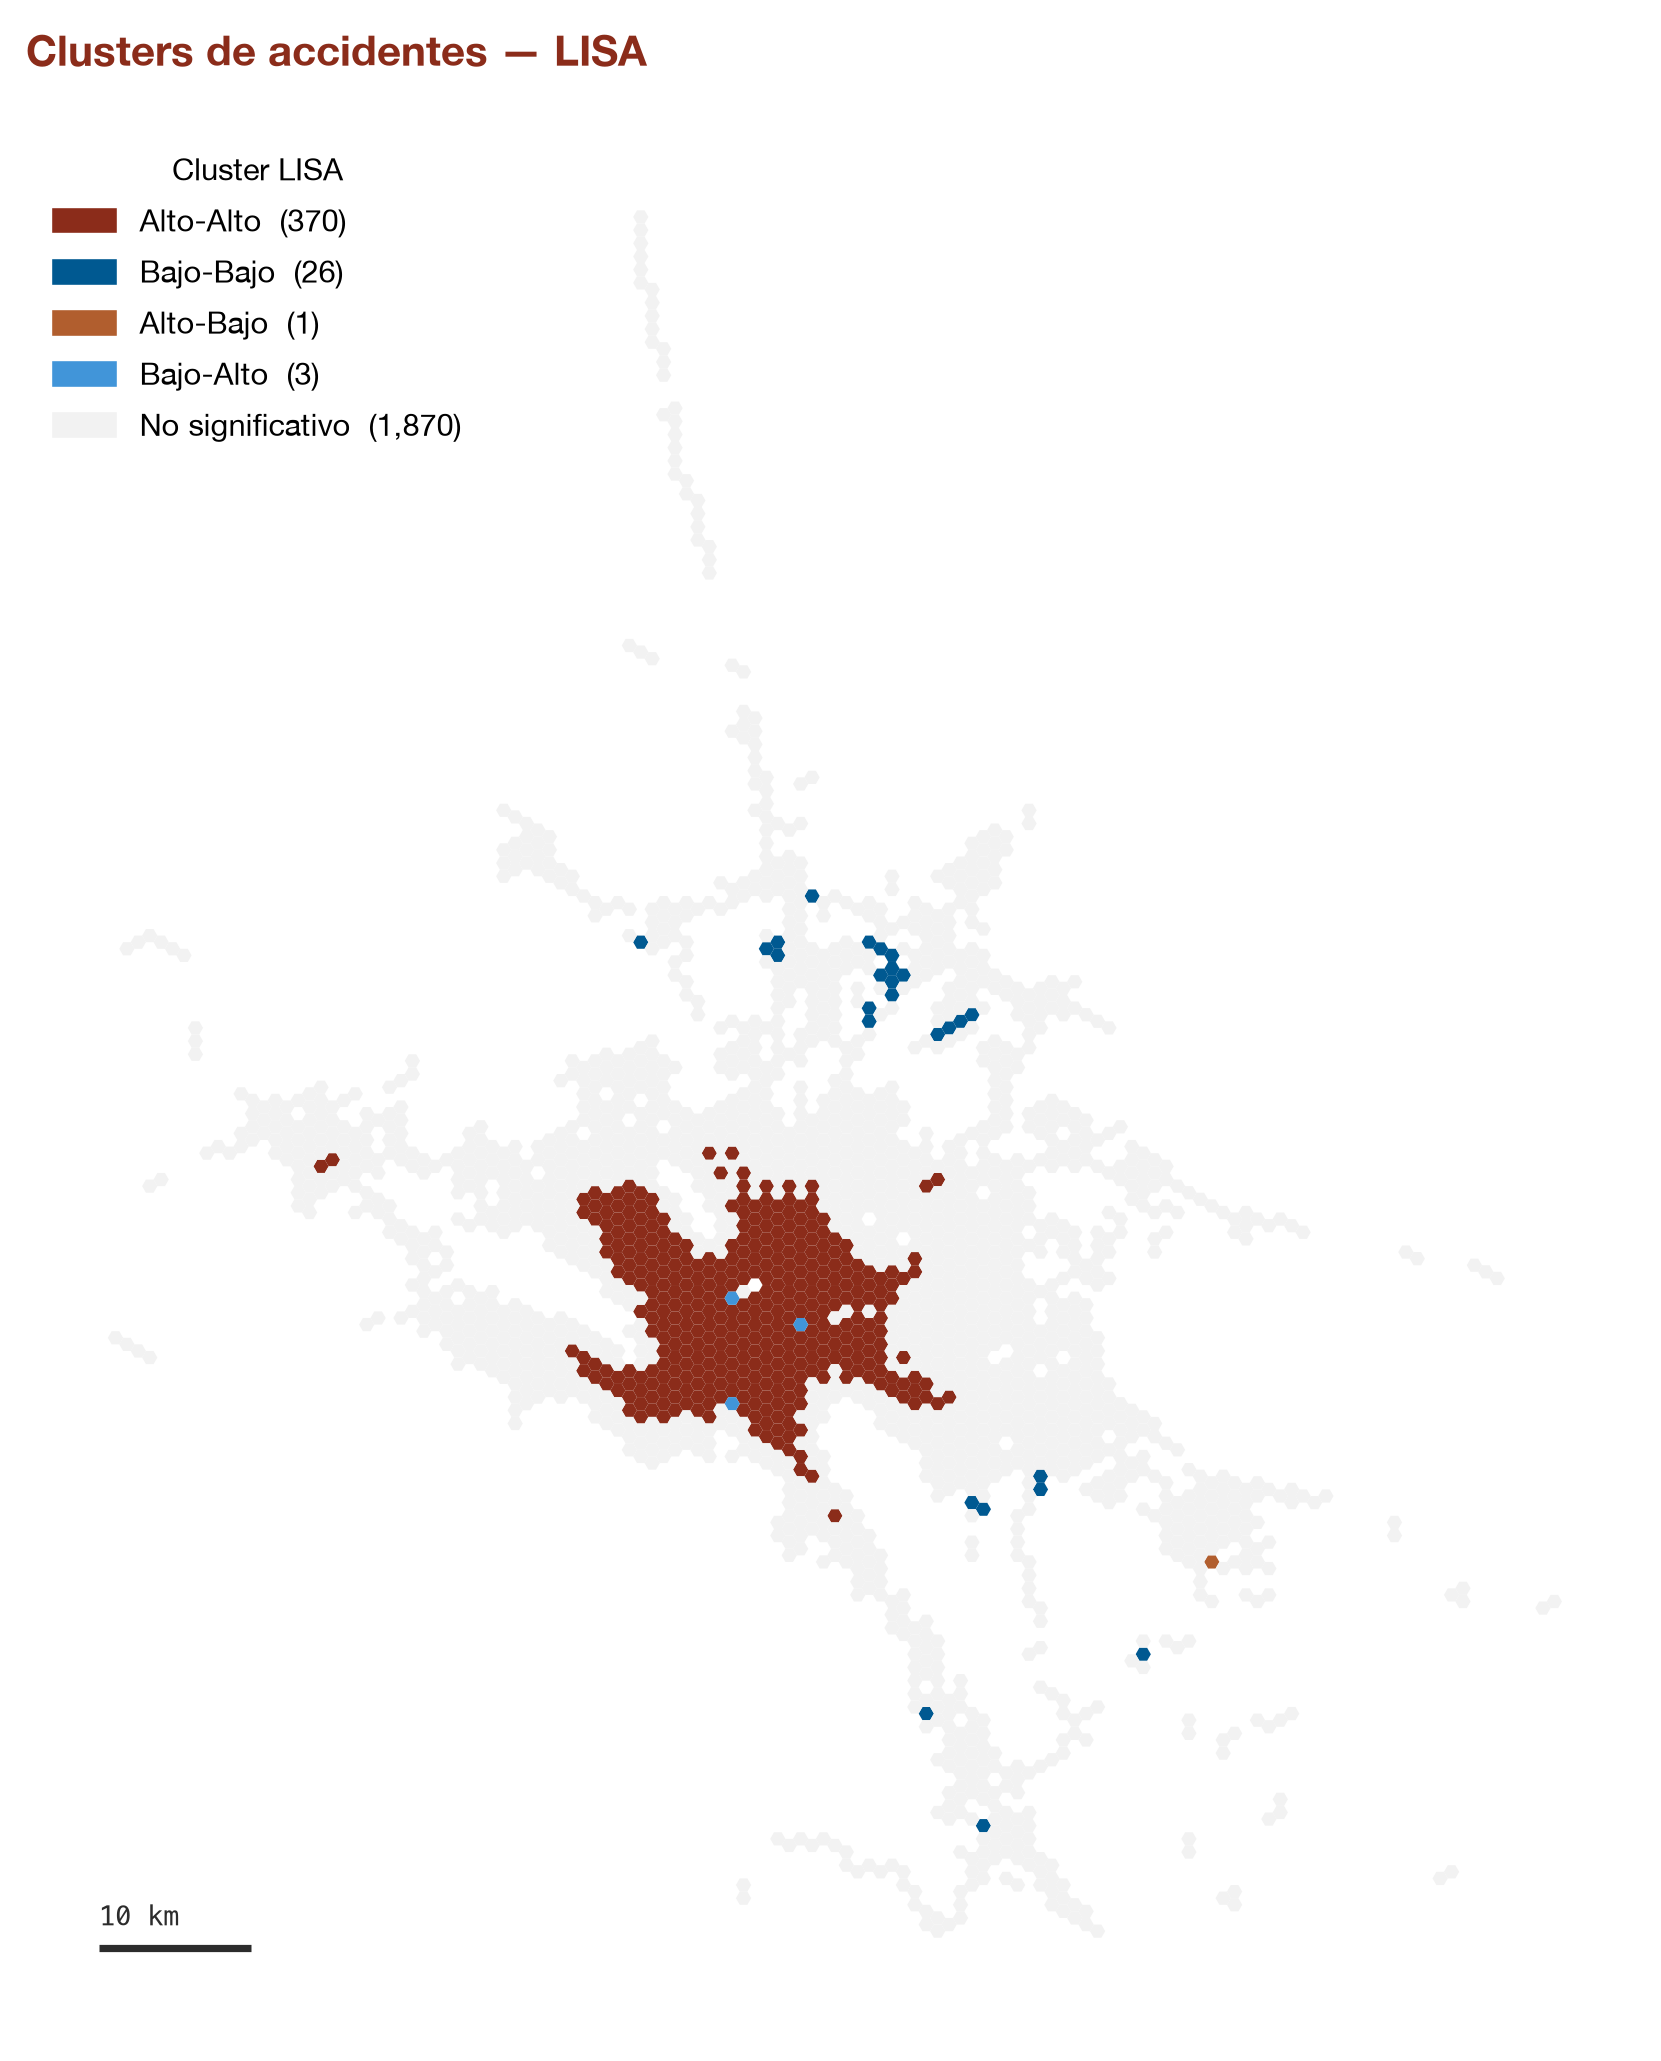
\includegraphics[width=0.45\textwidth]{lisa}\hfill
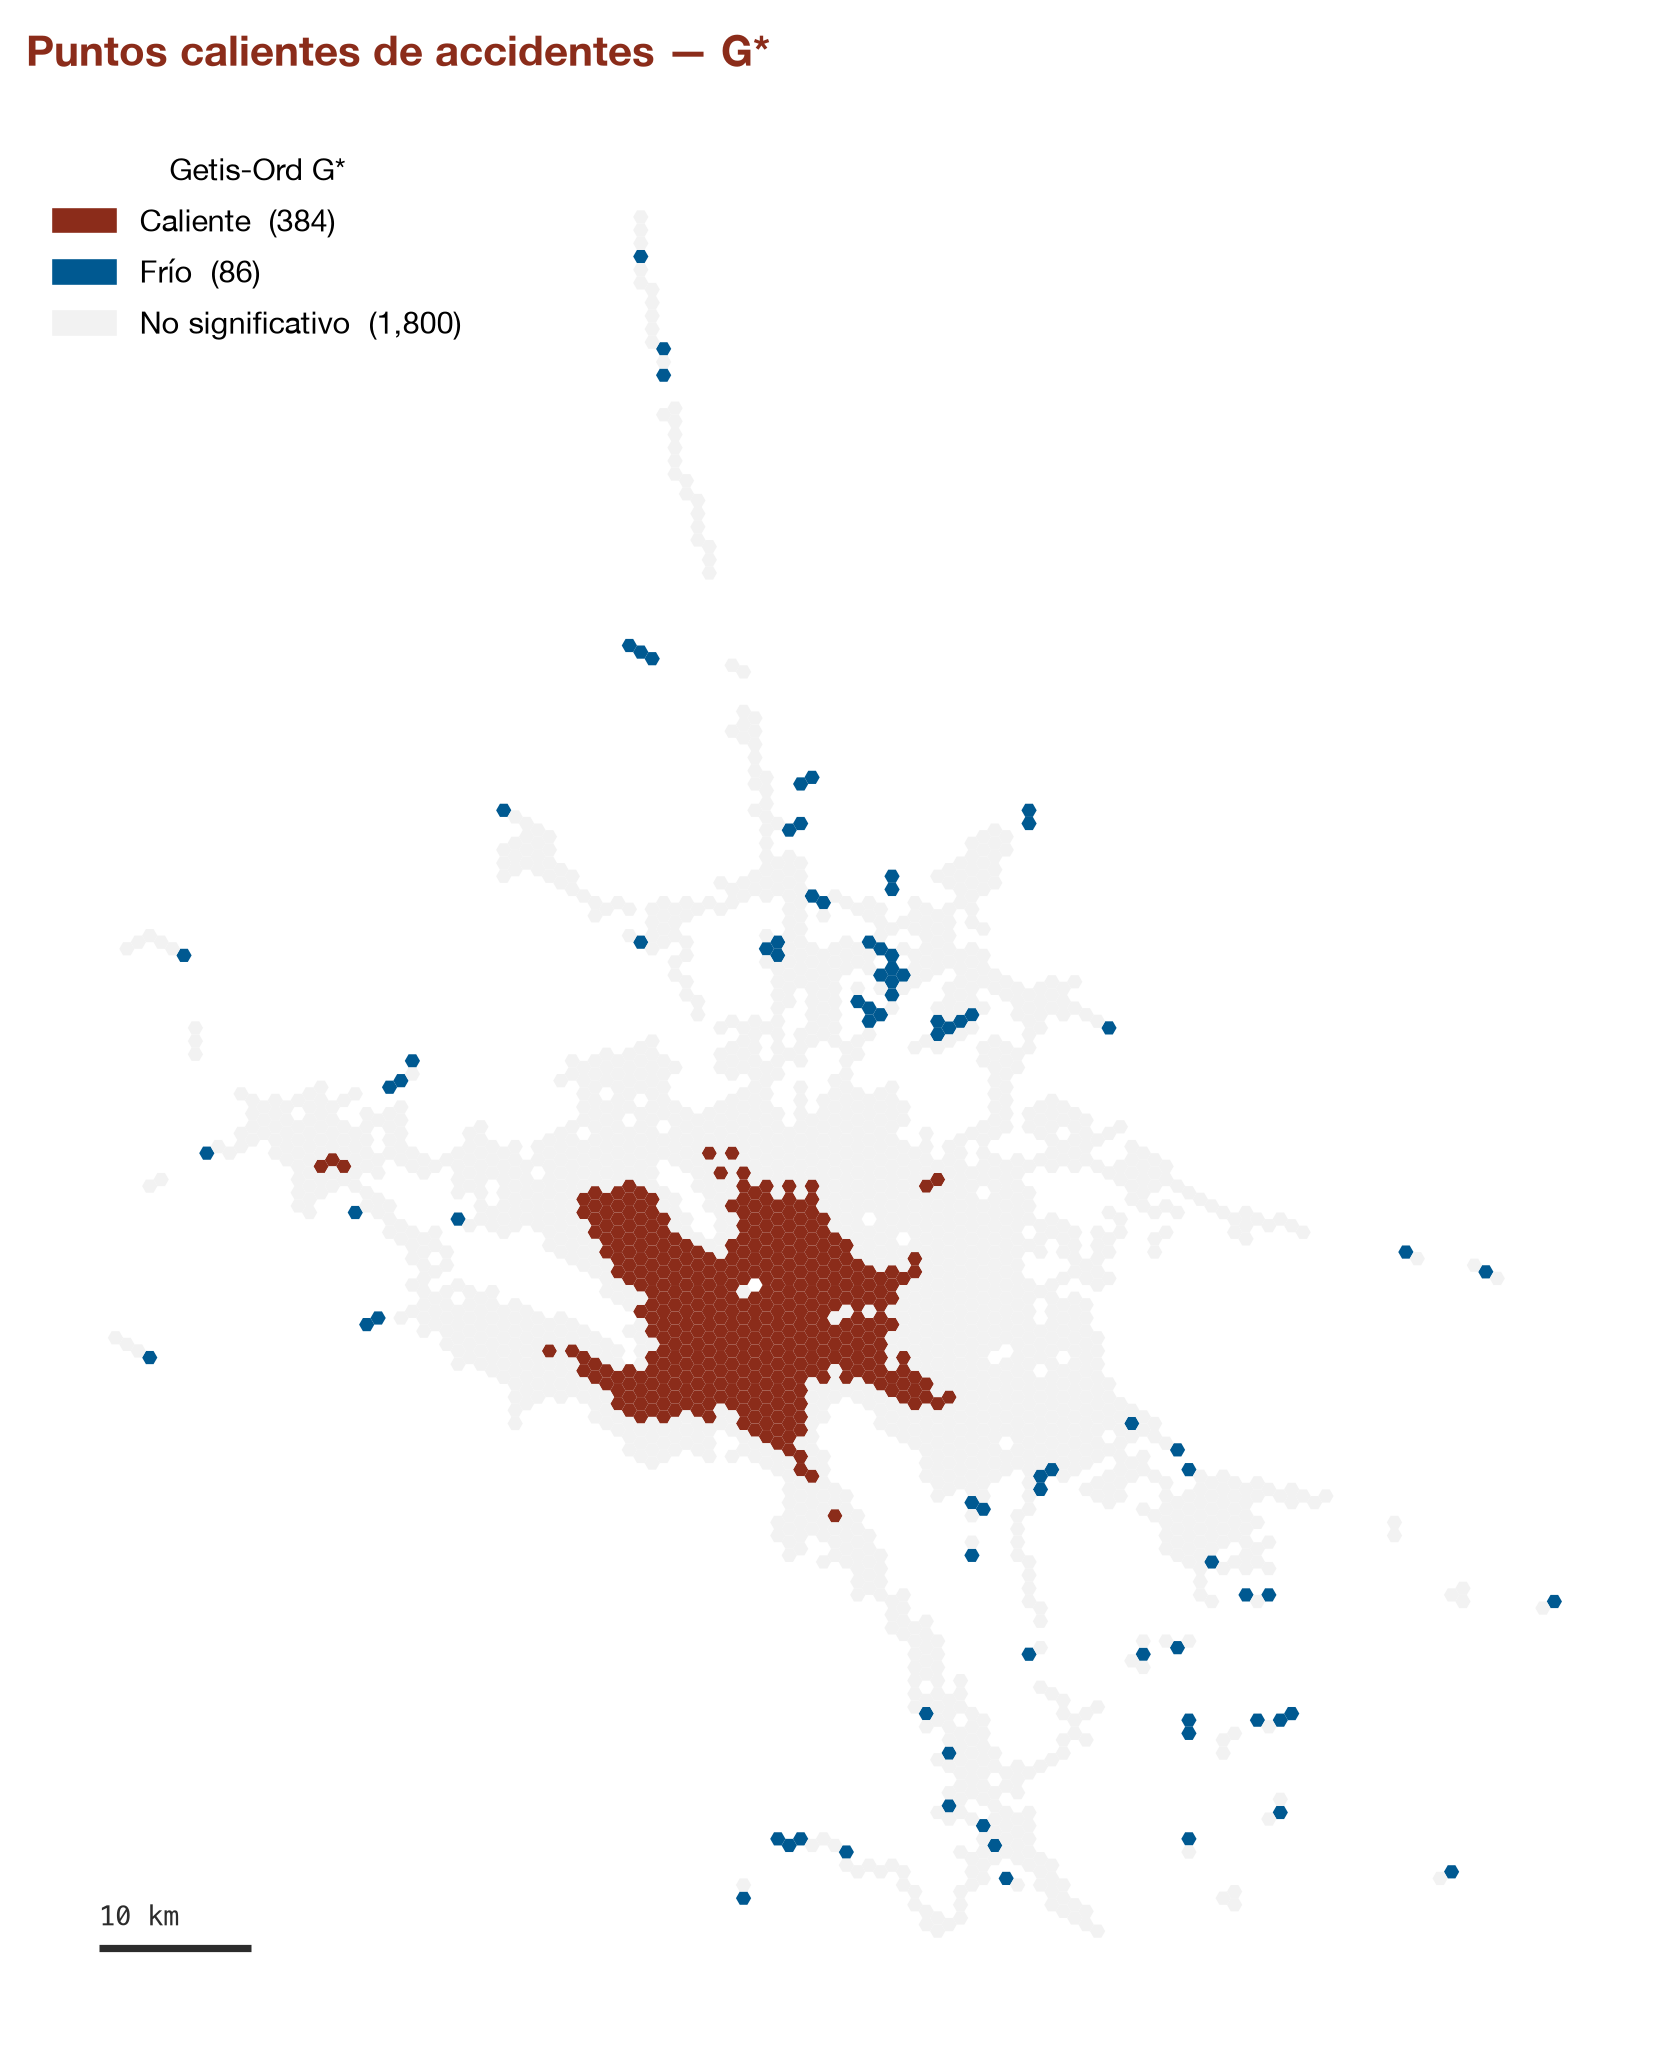
\includegraphics[width=0.45\textwidth]{gistar}
\caption{Izquierda: clusters LISA. Derecha: puntos calientes y fríos del
$G^*_i$ de Getis--Ord. Ambos con control de la tasa de falsos descubrimientos
al 5\,\%. Dos estadísticos con lógica distinta convergen en el mismo núcleo.}
\label{fig:res-local}
\end{figure*}

\paragraph{Persistencia.}
La estructura no es propia de un año. El $I$ de Moran anual se mantiene entre
0,60 y 0,69 de 2019 a 2024, y el ranking de celdas de 2019 tiene una
\textbf{correlación de Spearman de 0,83 con el de 2024}, con la pandemia de
por medio (figura~\ref{fig:res-persistencia}). La matriz de correlaciones
tiene además dos bloques: $\sim$0,90 dentro de 2019--2021 y dentro de
2022--2024, y $\sim$0,82 entre bloques. El corte coincide con la aparición del
campo \texttt{OID} en los archivos del INEGI a partir de 2022, lo que sugiere
un cambio en el procedimiento de georreferenciación; por eso los modelos
incluyen un indicador de periodo.

La prueba operativa de persistencia es el índice de precisión predictiva
(PAI) \citep{chainey_2008}: la fracción de accidentes capturada dividida
entre la fracción de territorio seleccionada. \textbf{Eligiendo el 5\,\% de
las celdas con más accidentes en 2019--2023 se captura el 42\,\% de los
accidentes de 2024: PAI de 8,4.} Este resultado no usa ningún modelo ---solo
contar y ordenar--- y es la referencia que cualquier modelo tiene que
superar.

\begin{figure*}
\centering
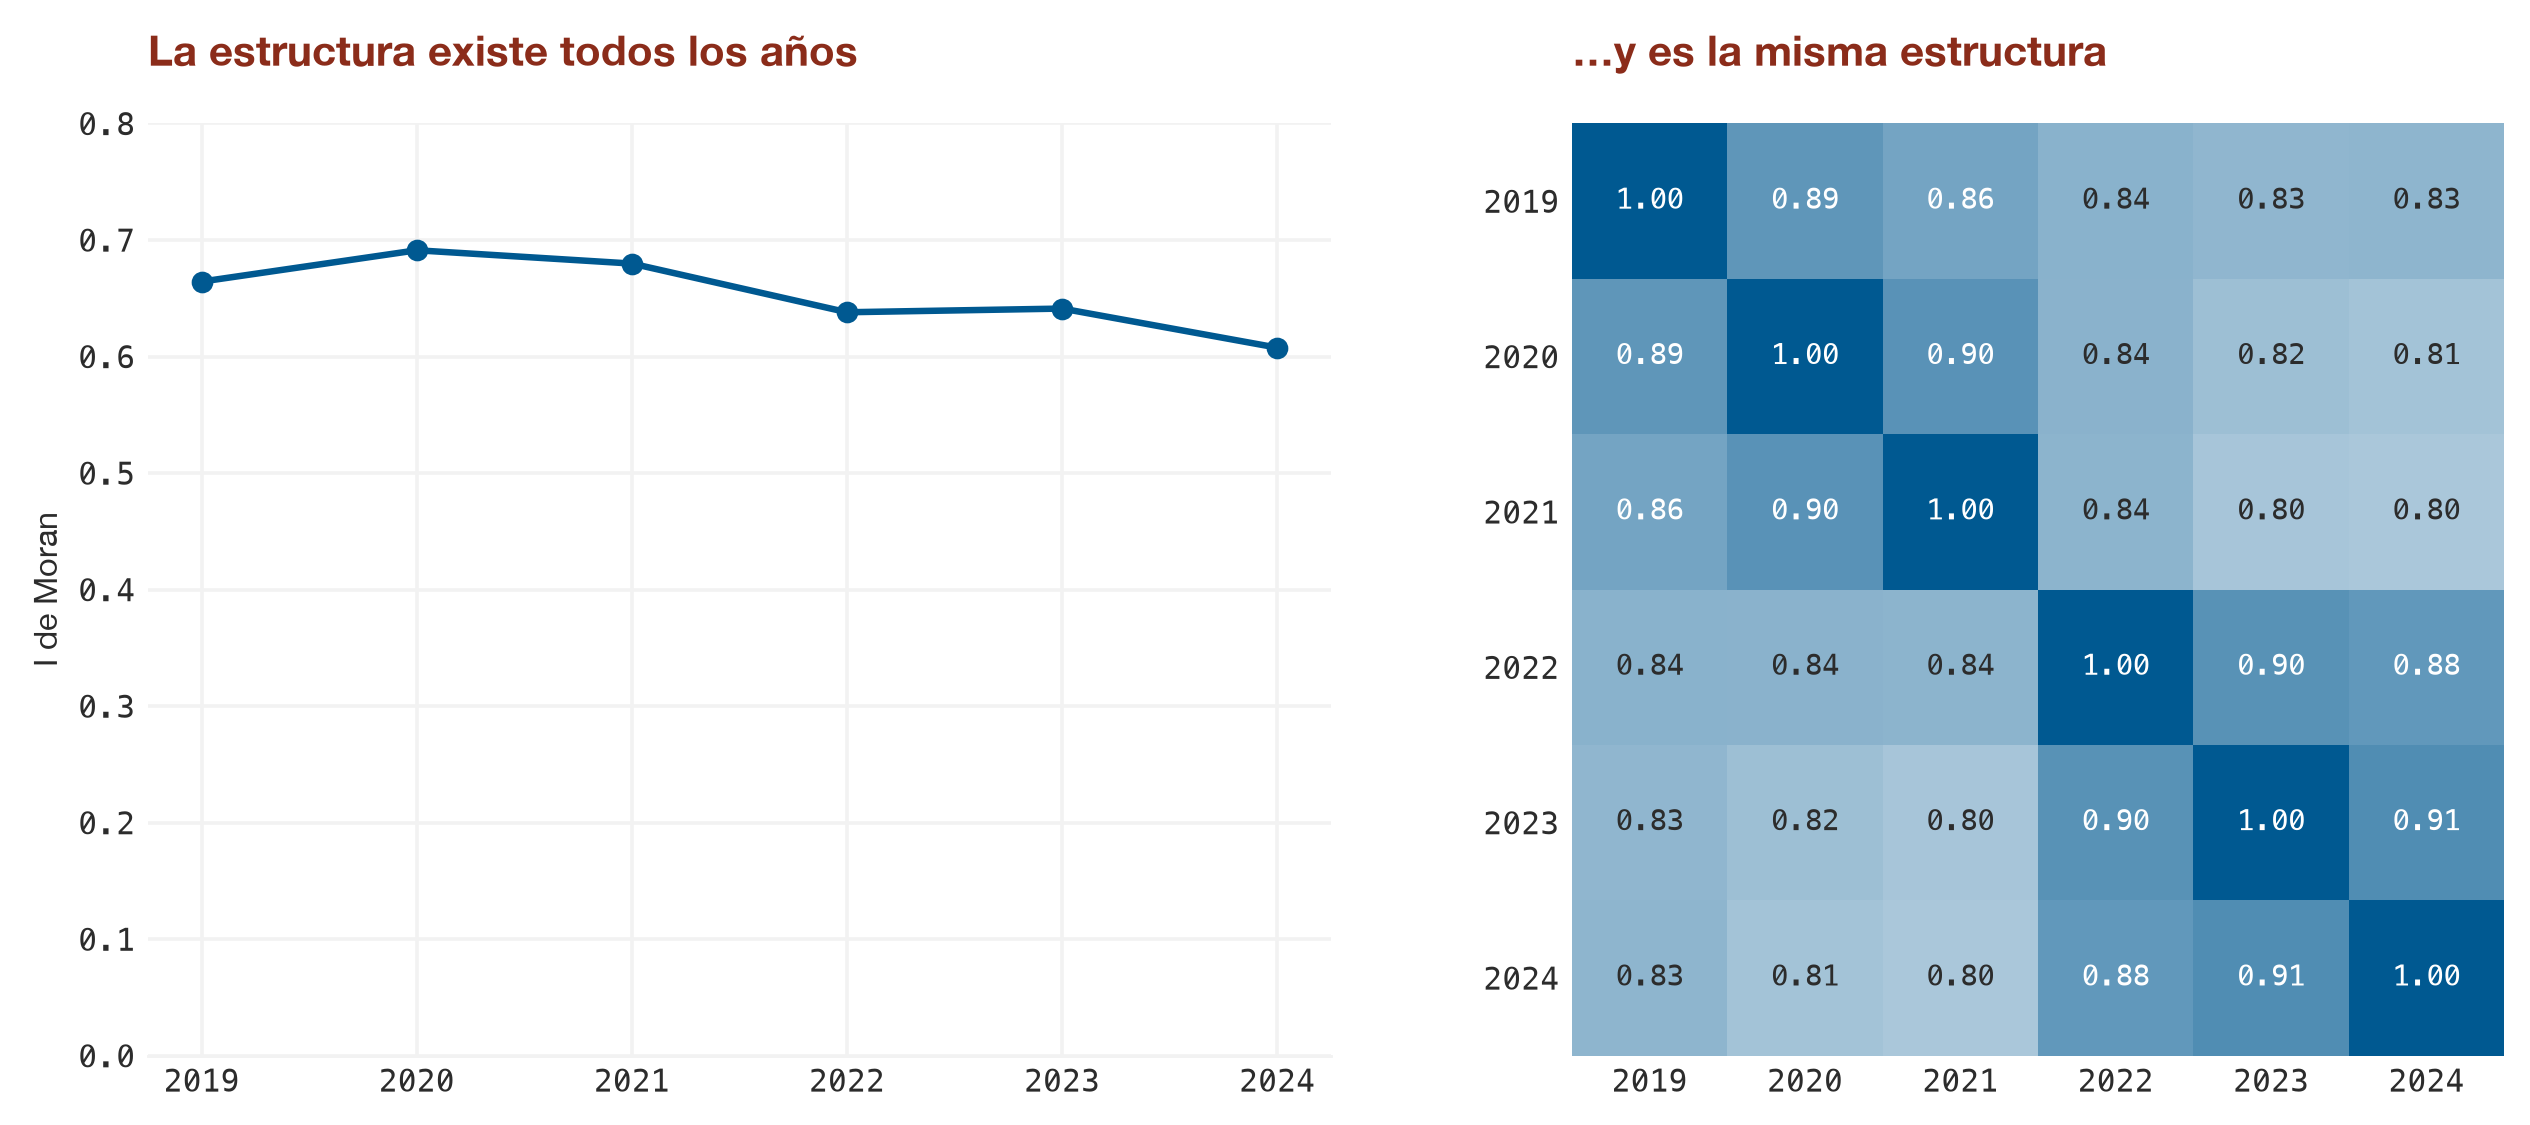
\includegraphics[width=0.85\textwidth]{persistencia}
\caption{Izquierda: $I$ de Moran por año. Derecha: correlación de Spearman
entre los conteos por celda de cada par de años; se distinguen los bloques
2019--2021 y 2022--2024.}
\label{fig:res-persistencia}
\end{figure*}

% ---------------------------------------------------------------------------
\subsection{Modelos de conteo}\label{sec:res-conteo}
% ---------------------------------------------------------------------------

\paragraph{Sobredispersión.}
En el panel de celda$\times$mes (161\,352 filas, 56\,\% de ceros) la razón
varianza/media marginal es 12,9. Condicionando en la historia de la celda,
$\log h_i$, el estadístico $\chi^2_{\text{Pearson}}/gl$ del GLM de Poisson
cae a 1,38: la historia absorbe casi toda la heterogeneidad, pero lo que
queda es inequívoco. La prueba de \citet{cameron_trivedi_1990} estima
$\hat\alpha = 0{,}096$ con $t = 59$. La Binomial Negativa NB2 estima
$\theta = 5{,}5$ y mejora el AIC en unos 13\,000 puntos respecto a Poisson y
en 600 respecto a NB1. Como $1/\theta = 0$ está en la frontera del espacio
paramétrico, la razón de verosimilitudes se evalúa contra una mezcla 50:50 de
una masa en cero y una $\chi^2_1$ \citep{self_liang_1987}; el rechazo de
Poisson se mantiene con cualquier convención.

El rootograma colgante \citep{kleiber_zeileis_2016} hace visible la
diferencia (figura~\ref{fig:res-rootograma}): Poisson subpredice los ceros en
unas 4\,500 celdas-mes y sobrepredice los unos en 2\,900; NB2 corrige casi
todo el desajuste. Los residuales cuantil aleatorizados de NB2 sobre 2024
\citep{dunn_smyth_1996} tienen desviación estándar de 1,12 en lugar de 1, con
una cola derecha más pesada que la normal (figura~\ref{fig:res-rqr}): queda
dispersión que el modelo no captura, y la sección siguiente muestra de dónde
viene.

\begin{figure*}
\centering
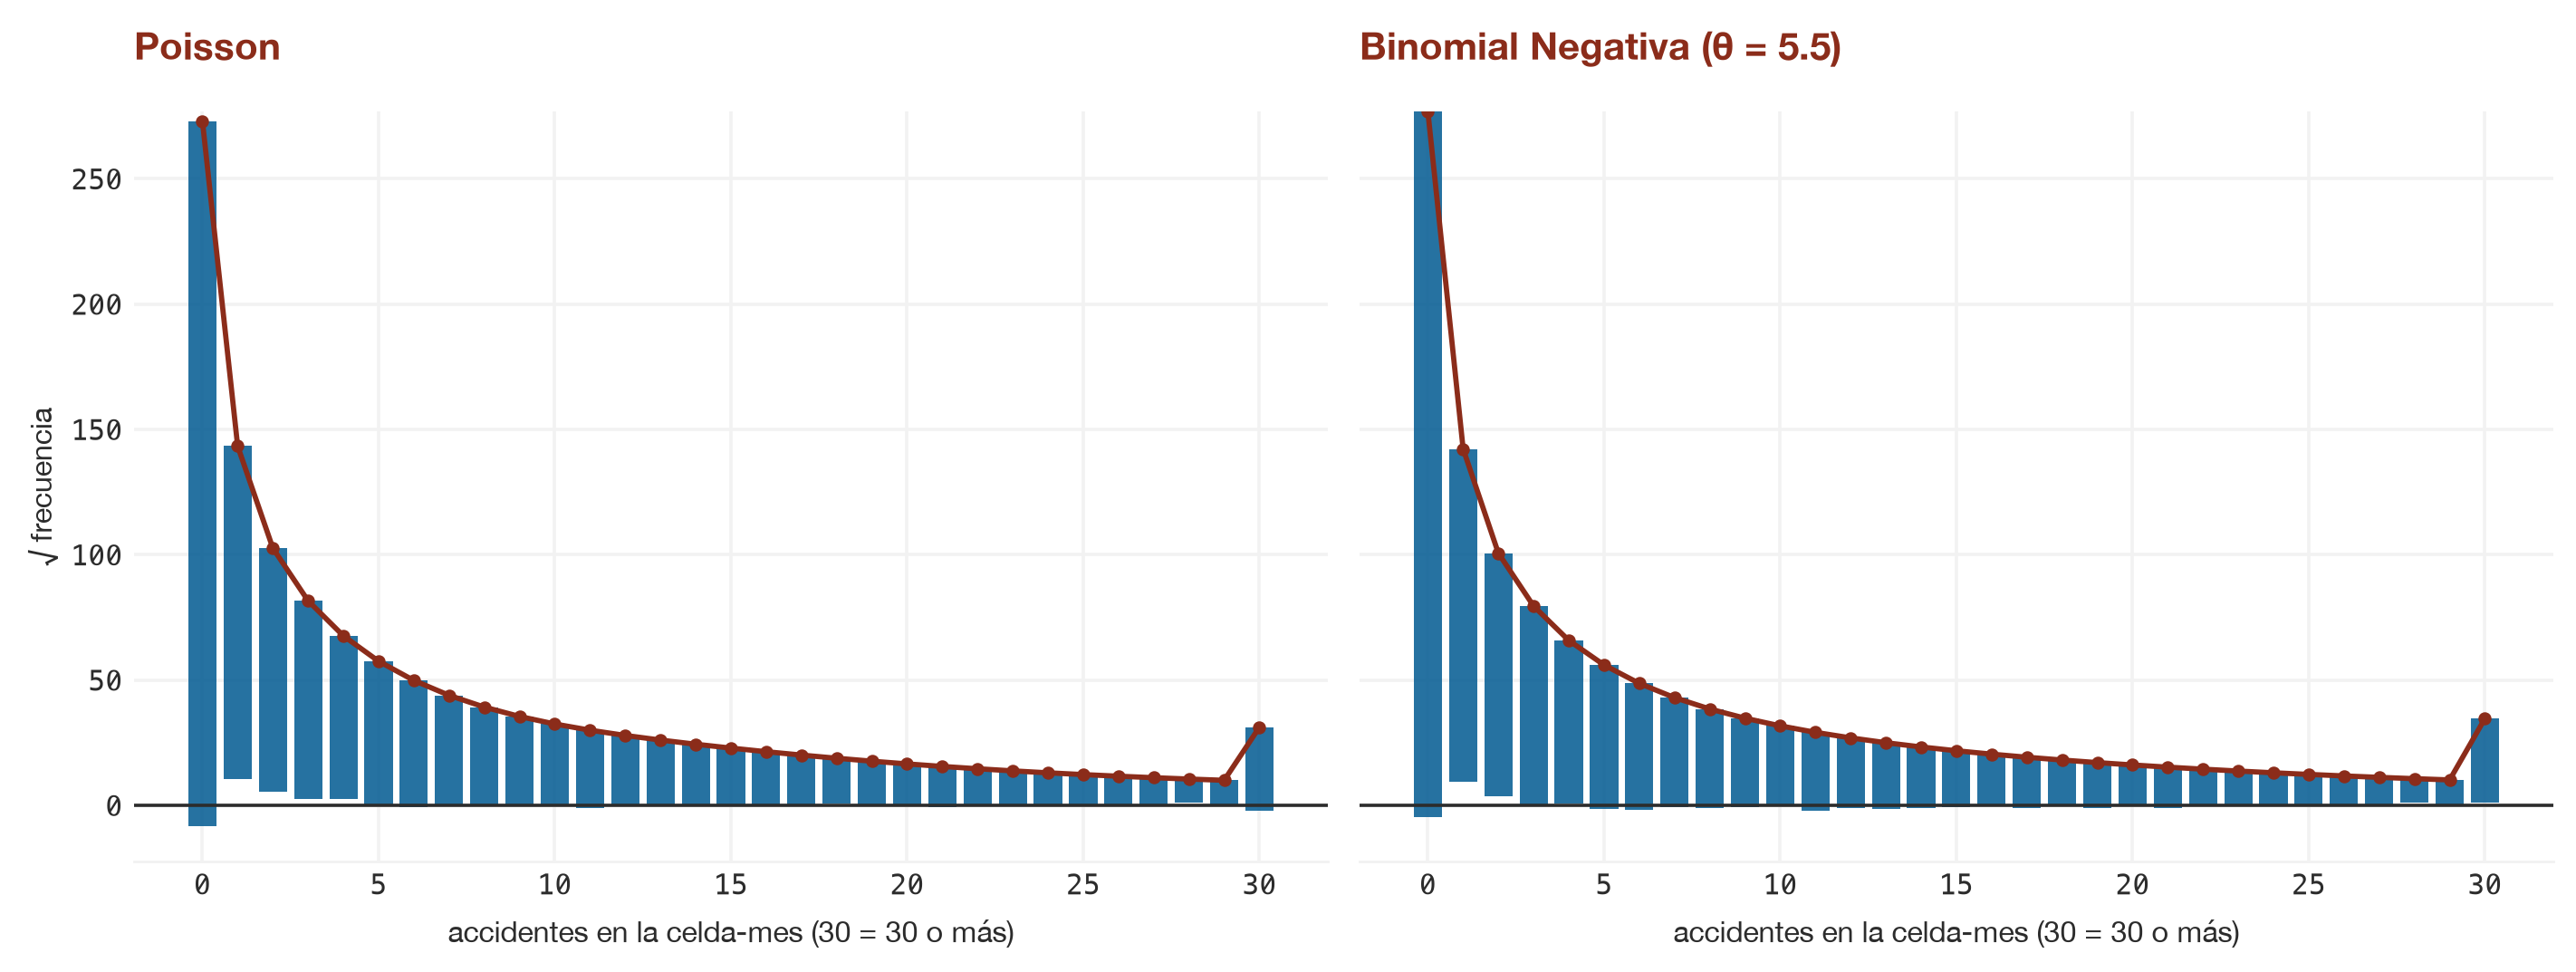
\includegraphics[width=0.85\textwidth]{rootograma}
\caption{Rootogramas colgantes de Poisson y NB2 en el panel
celda$\times$mes. Las barras cuelgan de la frecuencia esperada (línea); si su
base toca el cero, el modelo ajusta ese valor.}
\label{fig:res-rootograma}
\end{figure*}

\begin{figure*}
\centering
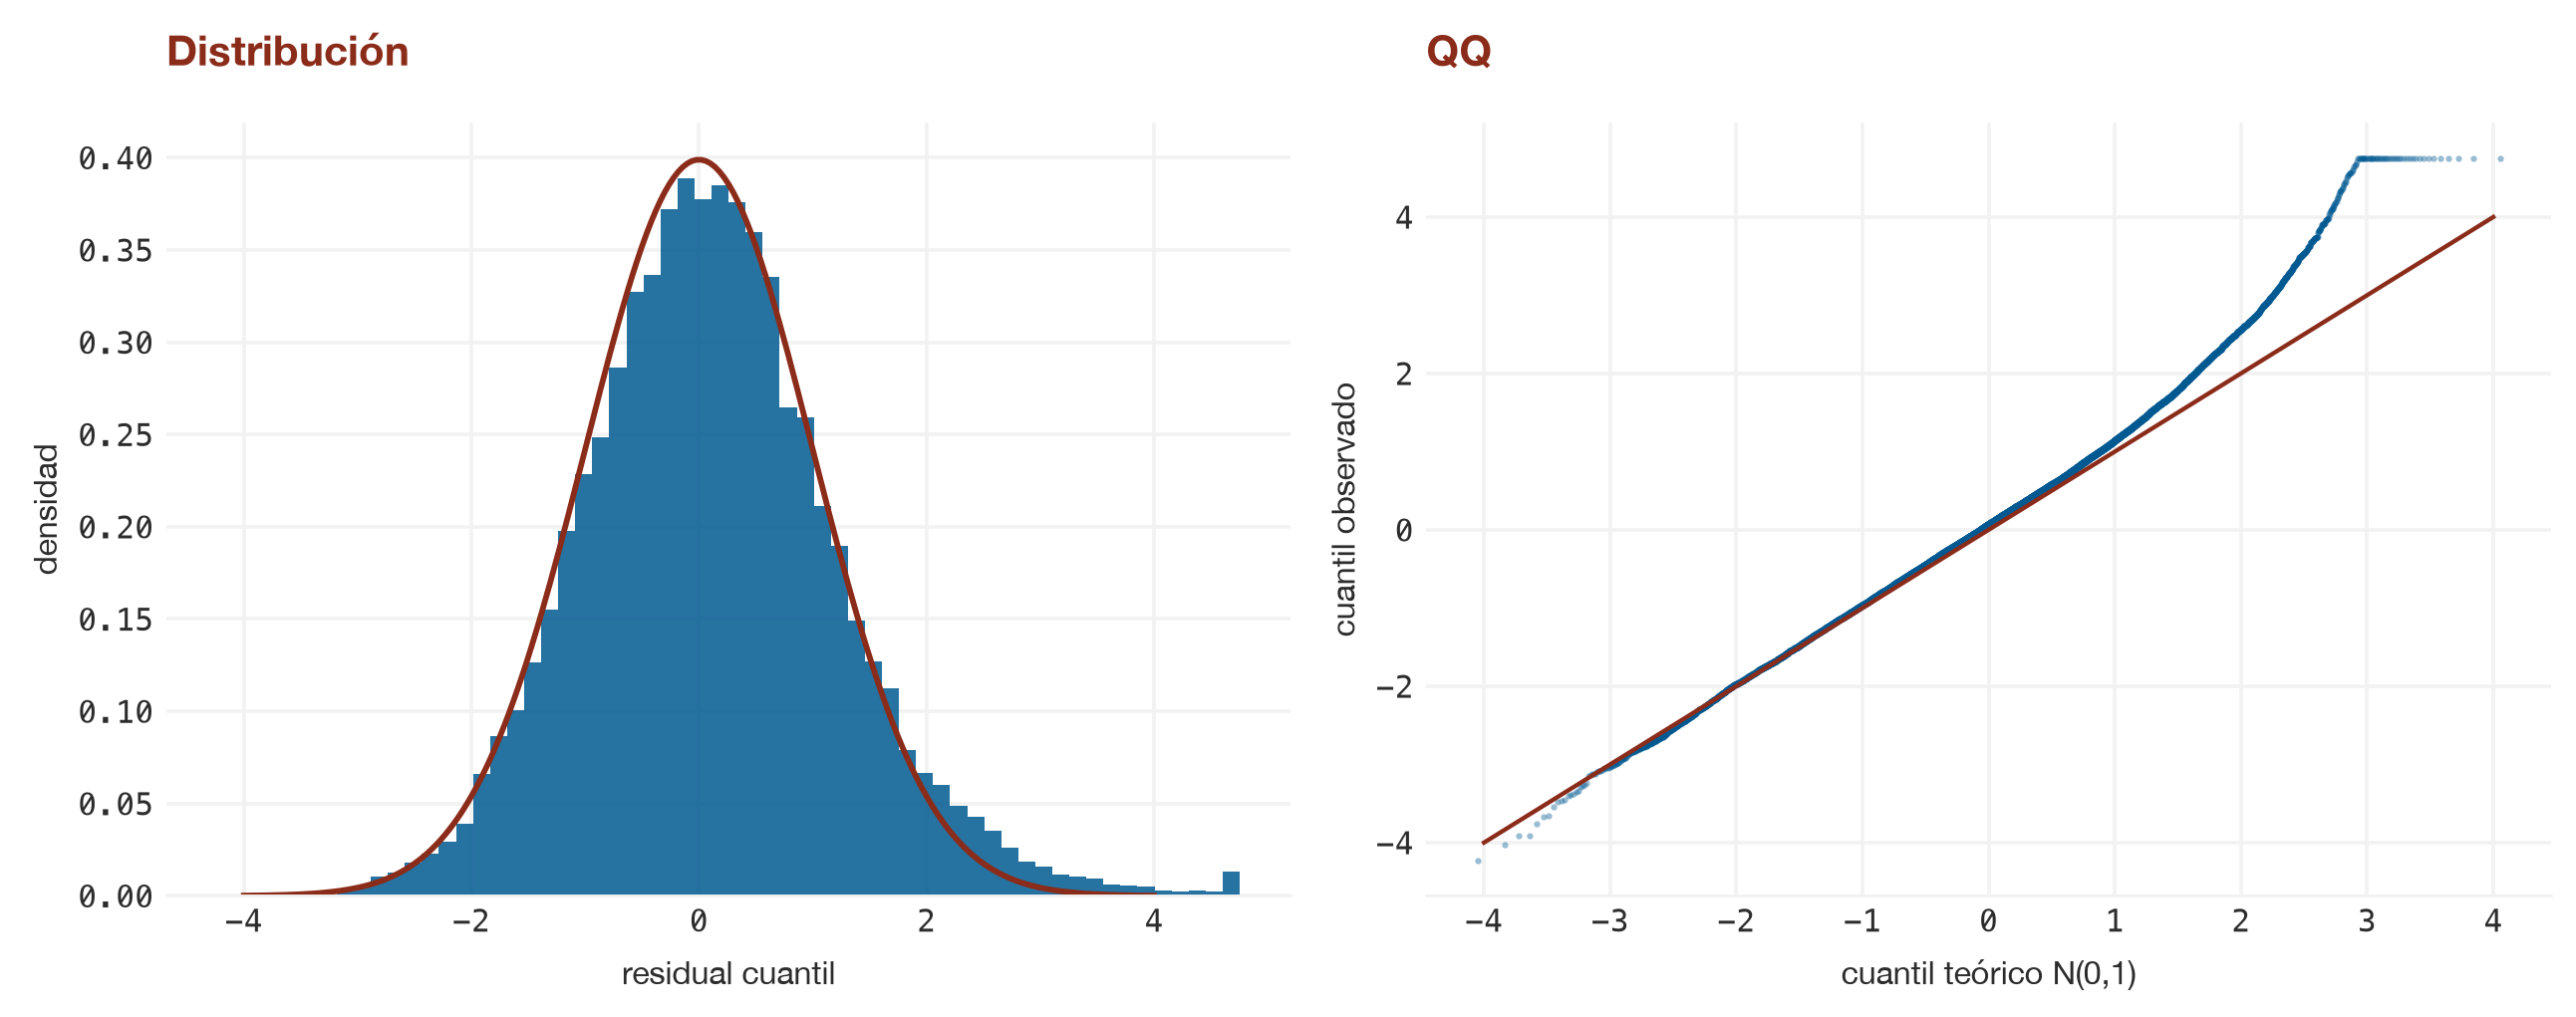
\includegraphics[width=0.85\textwidth]{rqr}
\caption{Residuales cuantil aleatorizados de NB2 sobre 2024: histograma
frente a la densidad $N(0,1)$ y gráfico QQ. La desviación se concentra en la
cola superior.}
\label{fig:res-rqr}
\end{figure*}

\paragraph{Exceso de ceros.}
A NB2 le falta el 3,3\,\% de los ceros. Un ZINB con inflación constante
estima $\hat\pi = 0{,}026$ y mejora el AIC en 1\,200, pero el exceso no está
repartido: ocho pares municipio$\times$periodo explican dos tercios de él,
con Santa Catarina en prepandemia y pandemia a la cabeza. Ese municipio
registró 128, 3 y 77 accidentes en 2019, 2020 y 2021, y 1\,793 en 2022. Los
ceros ``estructurales'' son celdas de municipios que no reportaban, no
celdas sin riesgo, por lo que no se adoptó un modelo de inflación de ceros.

\paragraph{Comparación fuera de muestra.}
El cuadro~\ref{tab:res-conteo} resume la validación en 2024 de los modelos
de conteo a escala celda$\times$mes.

\begin{table*}
\centering\small
\caption{Validación en 2024 a escala celda$\times$mes. Devianza y MAE miden
el acierto en la media; CRPS y cobertura, en la distribución; PAI, en la
selección del 5\,\% de celdas. En negritas, el mejor CRPS.}
\label{tab:res-conteo}
\begin{tabular}{@{}lrrrrr@{}}
\toprule
Modelo & Devianza & MAE & CRPS & Cobertura 90\,\% & PAI 5\,\% \\
\midrule
M0: histórico 2019--2023          & 40\,737 & 1,246 & 0,909 & 89,8\,\% & 8,41 \\
M0r: histórico 2022--2023         & 35\,652 & 1,196 & \textbf{0,844} & 92,0\,\% & 8,38 \\
M1: Poisson                       & 39\,705 & 1,247 & 0,895 & 90,2\,\% & 8,41 \\
M2: NB2                           & 39\,701 & 1,254 & 0,886 & 93,9\,\% & 8,41 \\
M3: NB2 + rezago espacial         & 39\,702 & 1,254 & 0,886 & 93,9\,\% & 8,41 \\
M4: NB2, historia 2022--2023      & 35\,701 & 1,200 & 0,847 & 92,0\,\% & 8,38 \\
\bottomrule
\end{tabular}
\end{table*}

Cuatro resultados se desprenden de esta comparación:

\begin{enumerate}
\item \textbf{El PAI es idéntico en M0--M3.} Con $\beta_h = 1{,}01$ y
  covariables que solo varían en el tiempo, la predicción de cada celda es
  $h_i$ multiplicada por un factor común, y el ranking de celdas coincide con
  el del histórico (Spearman $= 1{,}000$). Un GLM con covariables temporales
  cambia el \emph{cuánto} y la incertidumbre, pero no el \emph{dónde}.
\item \textbf{El rezago espacial no aporta nada}: su coeficiente es
  $-0{,}002$ ($t = -0{,}6$), pese a la autocorrelación de 0,65 en los
  conteos.
\item \textbf{Dos años recientes predicen mejor que cinco}: el CRPS de M4 es
  0,847 contra 0,886 de M2, y el promedio simple de 2022--2023 (M0r) es el
  mejor de la tabla. Cuando el modelo recibe ambas historias elige la
  completa, porque en entrenamiento explica mejor 2019--2021 al contenerlos;
  solo la validación fuera de muestra revela que generaliza peor.
\item \textbf{El residual tiene forma de municipio.} El $I$ de Moran del
  residual de NB2 en 2024 es 0,31 y cae a 0,07 al restar la media de cada
  municipio (figura~\ref{fig:res-municipal}). La autocorrelación residual no
  es un proceso espacial fino: son 18 bloques con un nivel propio. Por eso el
  rezago no ayudó: las vecinas de una celda de Guadalupe también están en
  Guadalupe y se equivocan en la misma dirección.
\end{enumerate}

\begin{figure*}
\centering
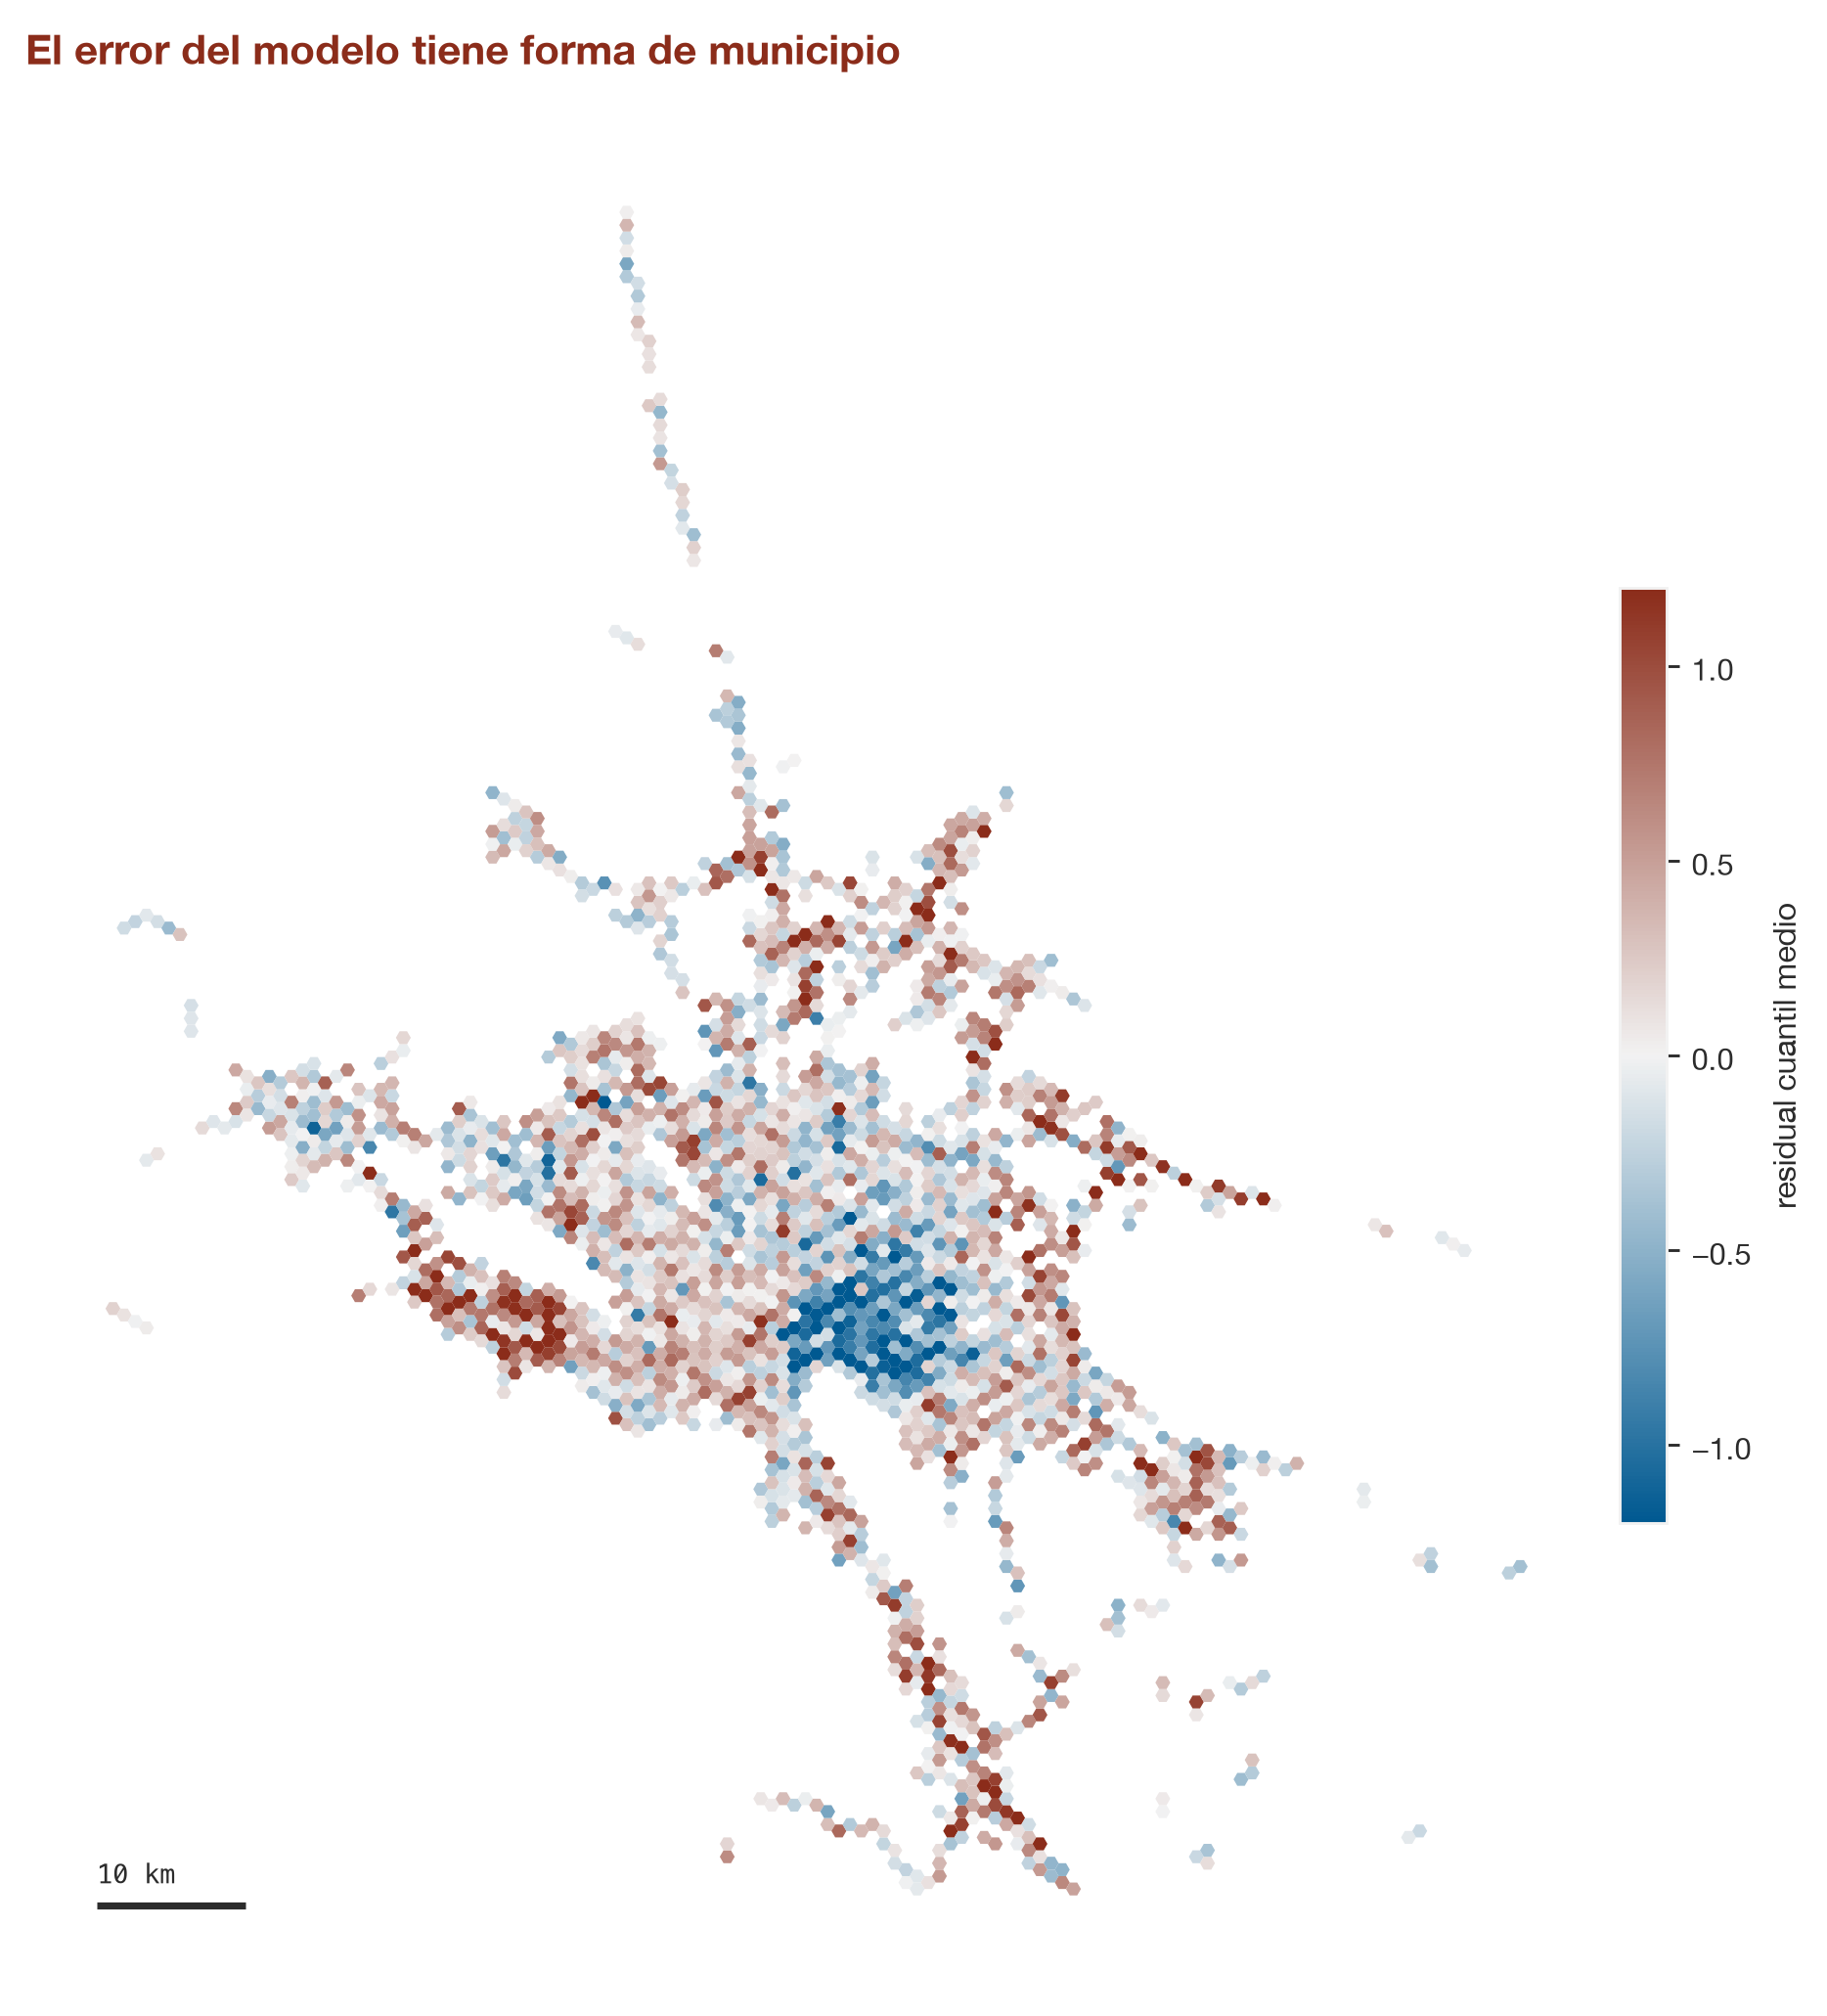
\includegraphics[width=0.42\textwidth]{residual_mapa}\hfill
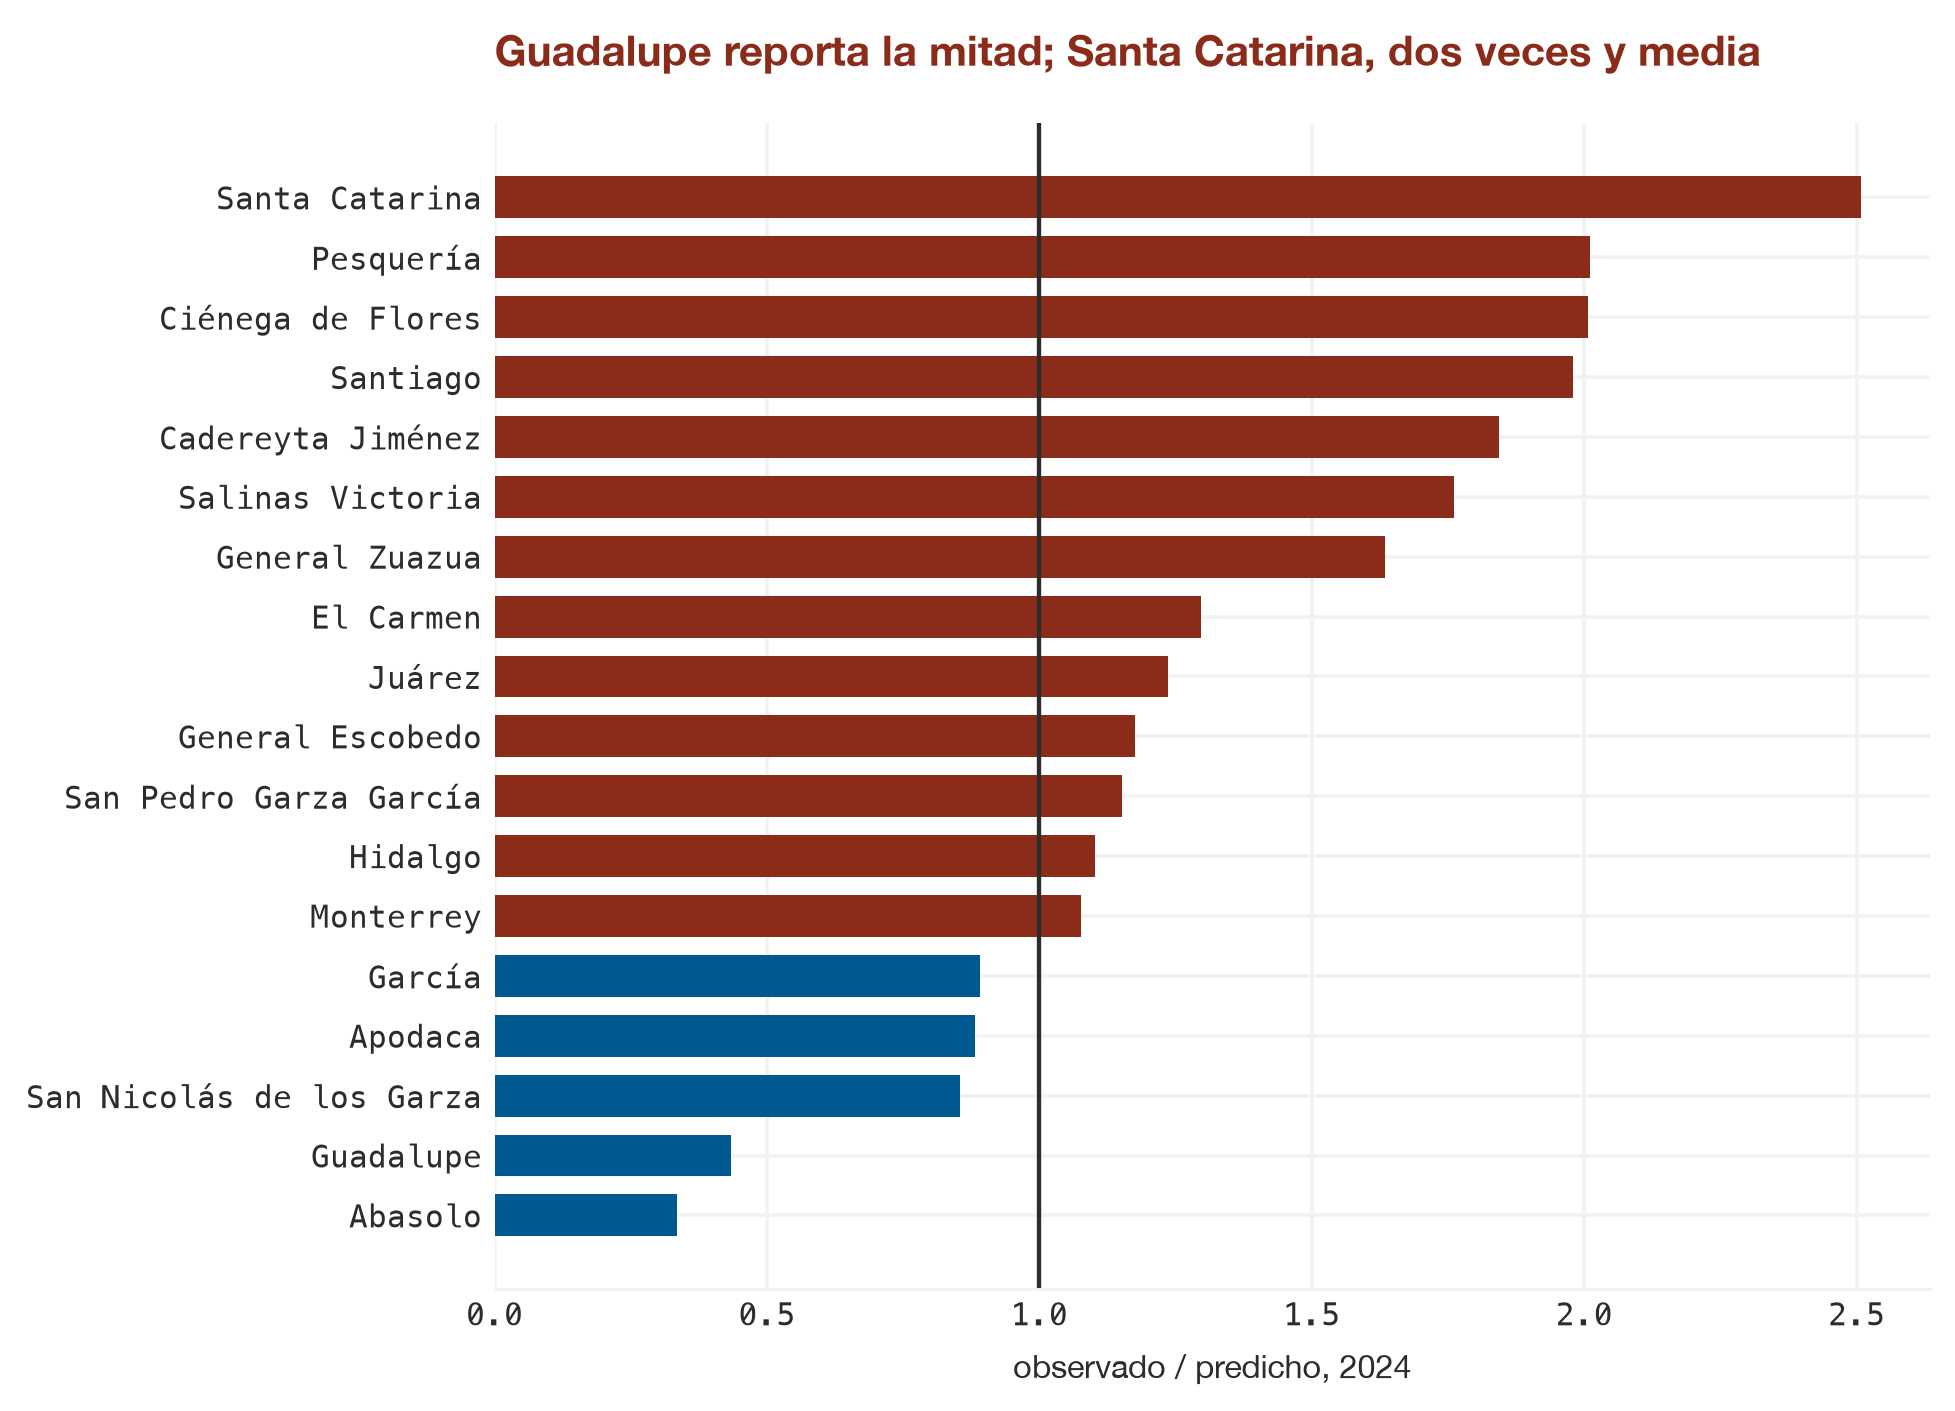
\includegraphics[width=0.52\textwidth]{cociente_municipal}
\caption{Izquierda: residual cuantil medio por celda en 2024 (NB2).
Derecha: cociente entre accidentes observados y predichos por municipio en
2024. Guadalupe registró el 43\,\% de lo que su historia predice; Santa
Catarina, 2,5 veces más.}
\label{fig:res-municipal}
\end{figure*}

Las series anuales por municipio (figura~\ref{fig:res-series}) explican el
patrón: Santa Catarina pasa de 3 accidentes en 2020 a 2\,904 en 2023;
Guadalupe alcanza su máximo en plena pandemia y cae a un tercio en 2024;
Salinas Victoria alterna 286, 827, 351 y 821. Ninguna dinámica vial produce
saltos de esa magnitud: lo que cambia de un año a otro es la práctica de
captura de cada municipio. El supuesto de subregistro estable no se sostiene,
y esta es la fuente dominante del error de predicción
(§\ref{sec:discusion}).

\begin{figure*}
\centering
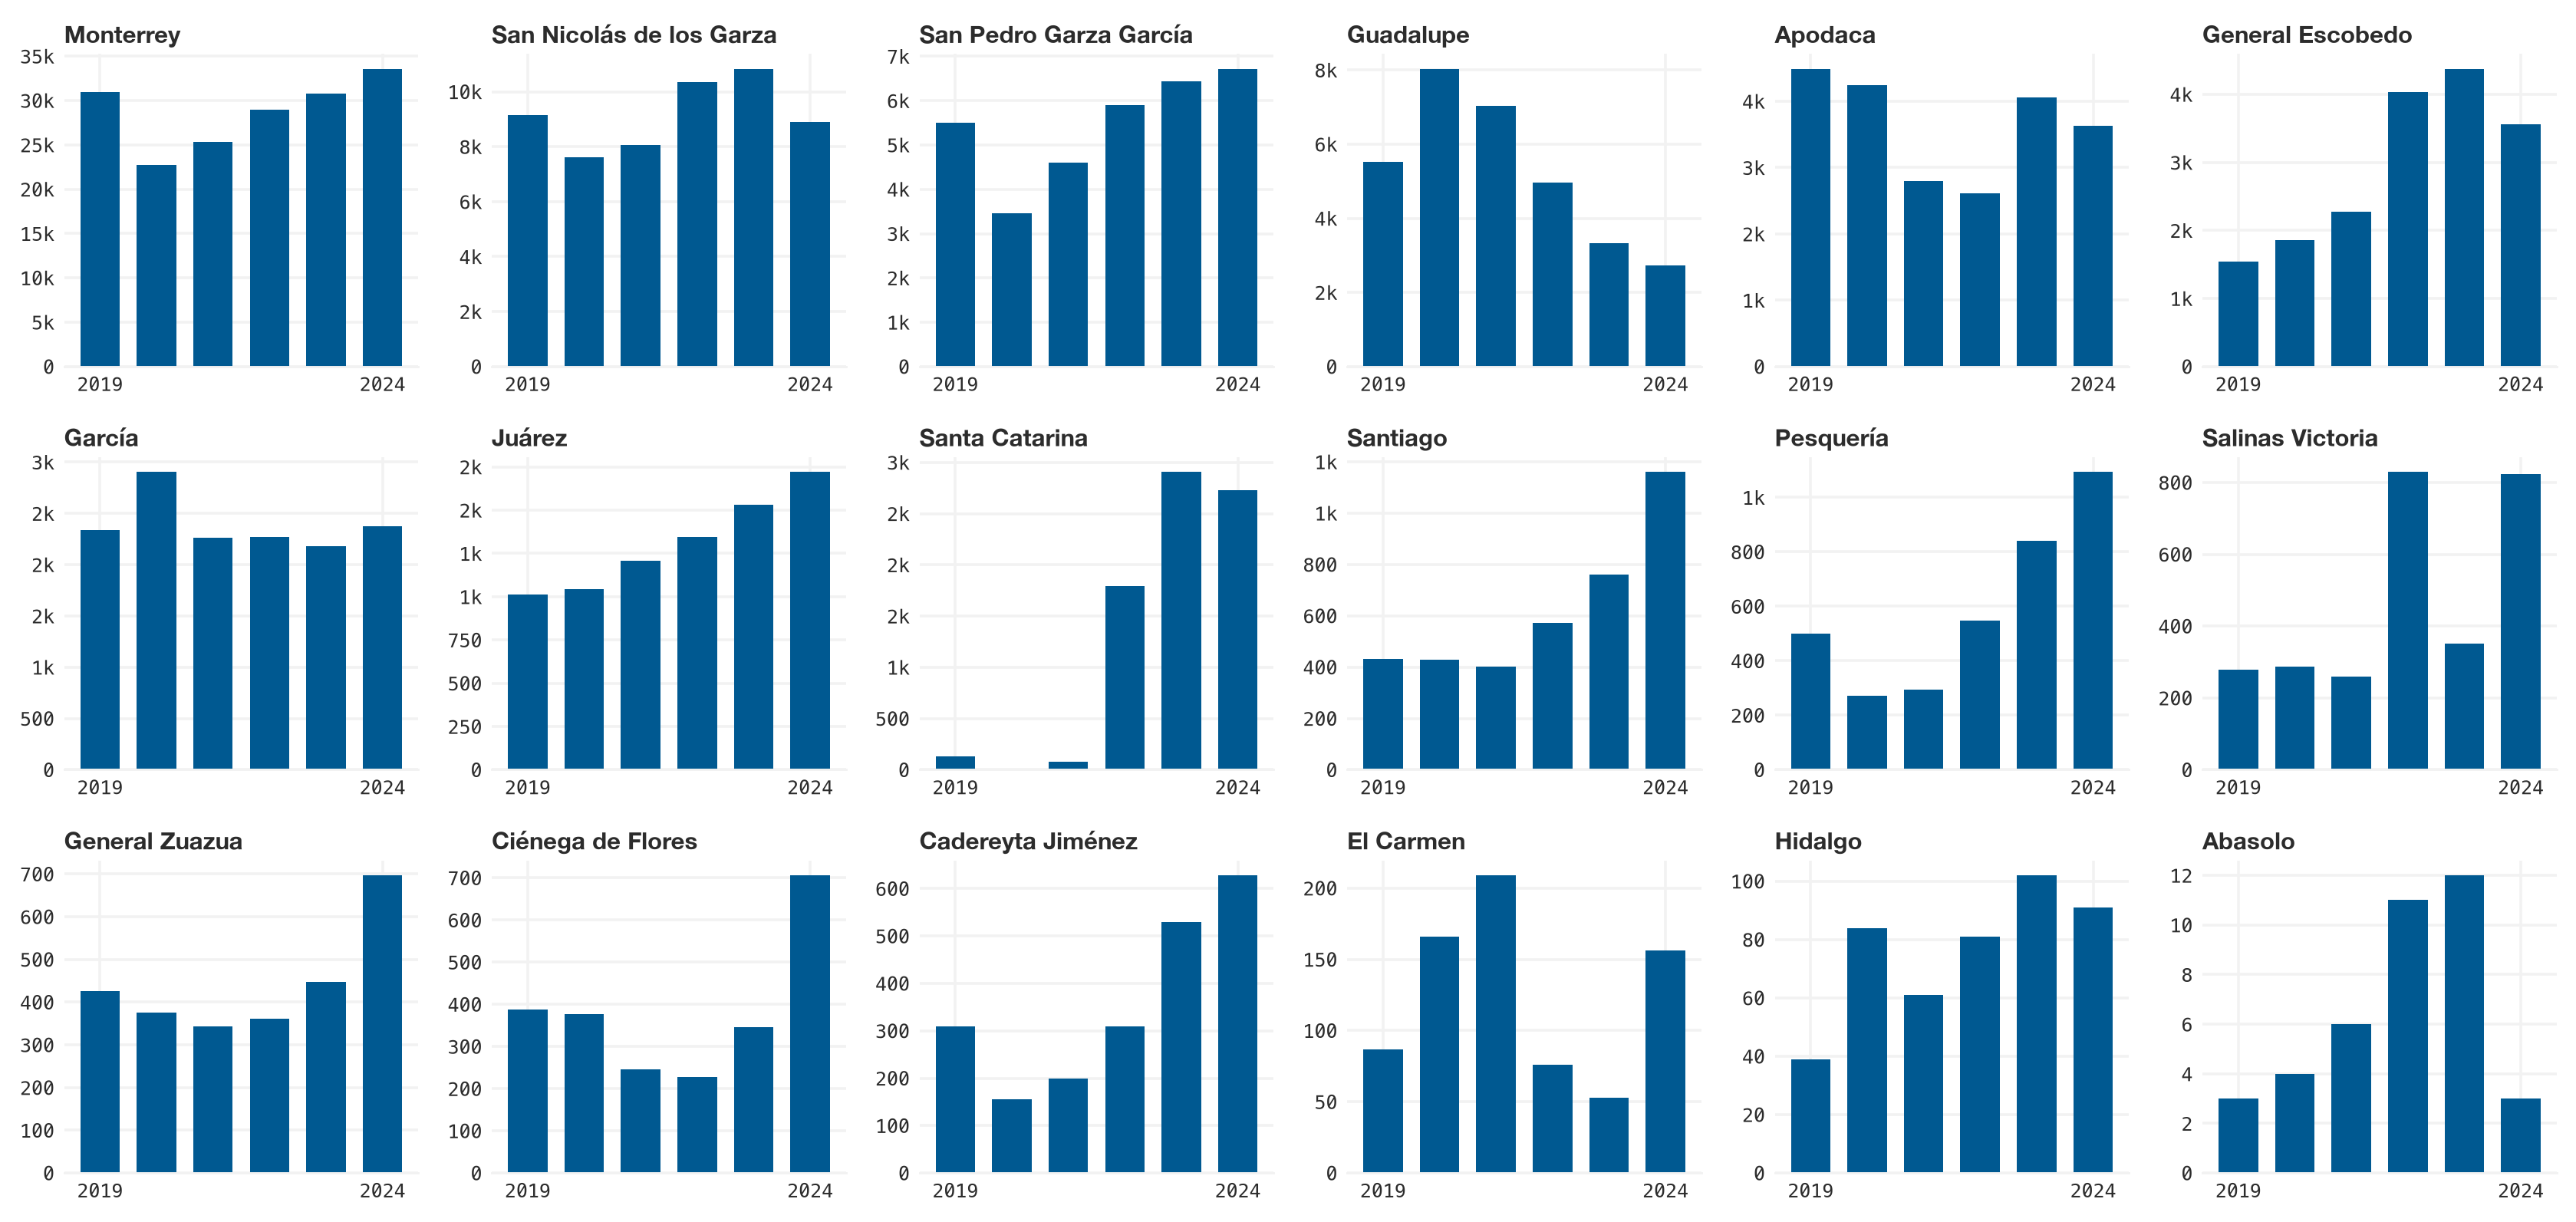
\includegraphics[width=\textwidth]{series_municipales}
\caption{Accidentes registrados por año en cada uno de los 18 municipios de
la ZMM, 2019--2024. Cada panel tiene su propia escala vertical.}
\label{fig:res-series}
\end{figure*}

% ---------------------------------------------------------------------------
\subsection{Modelo jerárquico}\label{sec:res-jerarquico}
% ---------------------------------------------------------------------------

\paragraph{BYM2 no se identifica.}
La especificación con efecto espacial BYM2 \citep{riebler_2016} se ajustó en
sus dos parametrizaciones y ninguna convergió
(cuadro~\ref{tab:res-bym2}). En la no centrada, la fracción espacial colapsa
a $\phi \to 0{,}0001$; en la centrada, $\sigma_s \to 13$ y
$\phi \to 0{,}9998$. Con cinco años de conteos por celda los datos fijan cada
$u_i$ casi por completo, y su reparto entre componente espacial e
independiente solo lo sostienen los priors. La estructura espacial existe ---el
$I$ de Moran de la tasa por celda, neta de la media municipal, es 0,41---, pero
no hay información para dividirla entre dos componentes. El modelo final usa
un CAR propio, con una sola varianza y un solo parámetro de dependencia.

\begin{table}
\centering\small
\caption{Intentos de ajuste de BYM2.}
\label{tab:res-bym2}
\begin{tabular}{@{}lp{3.6cm}r@{}}
\toprule
Parametrización & Resultado & $\hat{R}(\phi)$ \\
\midrule
No centrada & $\phi \to 0{,}0001$: desaparece la parte espacial & 2,06 \\
Centrada    & $\phi \to 0{,}9998$, $\sigma_s \to 13$: desaparece la parte independiente & 1,65 \\
\bottomrule
\end{tabular}
\end{table}

\paragraph{Diagnósticos de convergencia.}
El modelo final (cuatro cadenas NUTS con \texttt{nutpie}, 1\,000 iteraciones
de calentamiento y 2\,000 muestras por cadena) se ajustó en cuatro minutos
\textbf{sin divergencias}. Sobre las 11\,205 cantidades $\log\mu_{ia}$ ---las
que el modelo identifica--- el $\hat{R}$ máximo \citep{vehtari_2021} es 1,005
y el tamaño efectivo de muestra mínimo es 2\,441. El intercepto $\beta_0$ y
$\sigma_m$ mezclan peor porque comparten información con el nivel medio de
$\mathbf{u}$; ninguna conclusión depende de ellos por separado.

\paragraph{Hiperparámetros.}
El cuadro~\ref{tab:res-hiper} resume la posterior. La dependencia espacial
neta del municipio es fuerte ($\alpha = 0{,}85$). La sobredispersión a escala
anual es moderada ($\theta = 12{,}2$, frente a 5,5 a escala mensual). El
municipio típico cambia su nivel de reporte en un factor de
$e^{0{,}29} \approx 1{,}34$ al año, y dentro de un mismo municipio las celdas
difieren en órdenes de magnitud ($\sigma_u = 2{,}38$). Al reajustar con priors
alternativos ($\alpha$ uniforme, $\sigma_u$ con escala doble, $\theta$ con
media 5 en lugar de 20) los cuatro valores cambian en el tercer decimal: los
datos dominan a los priors. Con innovaciones normales en la caminata
municipal, $\sigma_{rw}$ se estimaba en 0,61, inflada por unos pocos saltos;
con innovaciones $t_3$ baja a 0,29.

\begin{table}
\centering\small
\caption{Hiperparámetros a posteriori del modelo jerárquico.}
\label{tab:res-hiper}
\begin{tabular}{@{}lrl@{}}
\toprule
Parámetro & Media & IC 94\,\% \\
\midrule
$\alpha$       & 0,85 & [0,81;\ 0,88] \\
$\theta$       & 12,2 & \\
$\sigma_{rw}$  & 0,29 & \\
$\sigma_u$     & 2,38 & \\
\bottomrule
\end{tabular}
\end{table}

\paragraph{Trayectorias municipales.}
Los efectos $m_{j,a}$ reproducen las series observadas
(figura~\ref{fig:res-trayectorias}): el salto de Santa Catarina en 2022, el
descenso sostenido de Guadalupe desde 2020 y el pico aislado de Salinas
Victoria. El intervalo es angosto en los municipios grandes (Monterrey, San
Nicolás de los Garza) y ancho en los pequeños (Abasolo, Ciénega de Flores),
como corresponde a la cantidad de información de cada uno.

\begin{figure*}
\centering
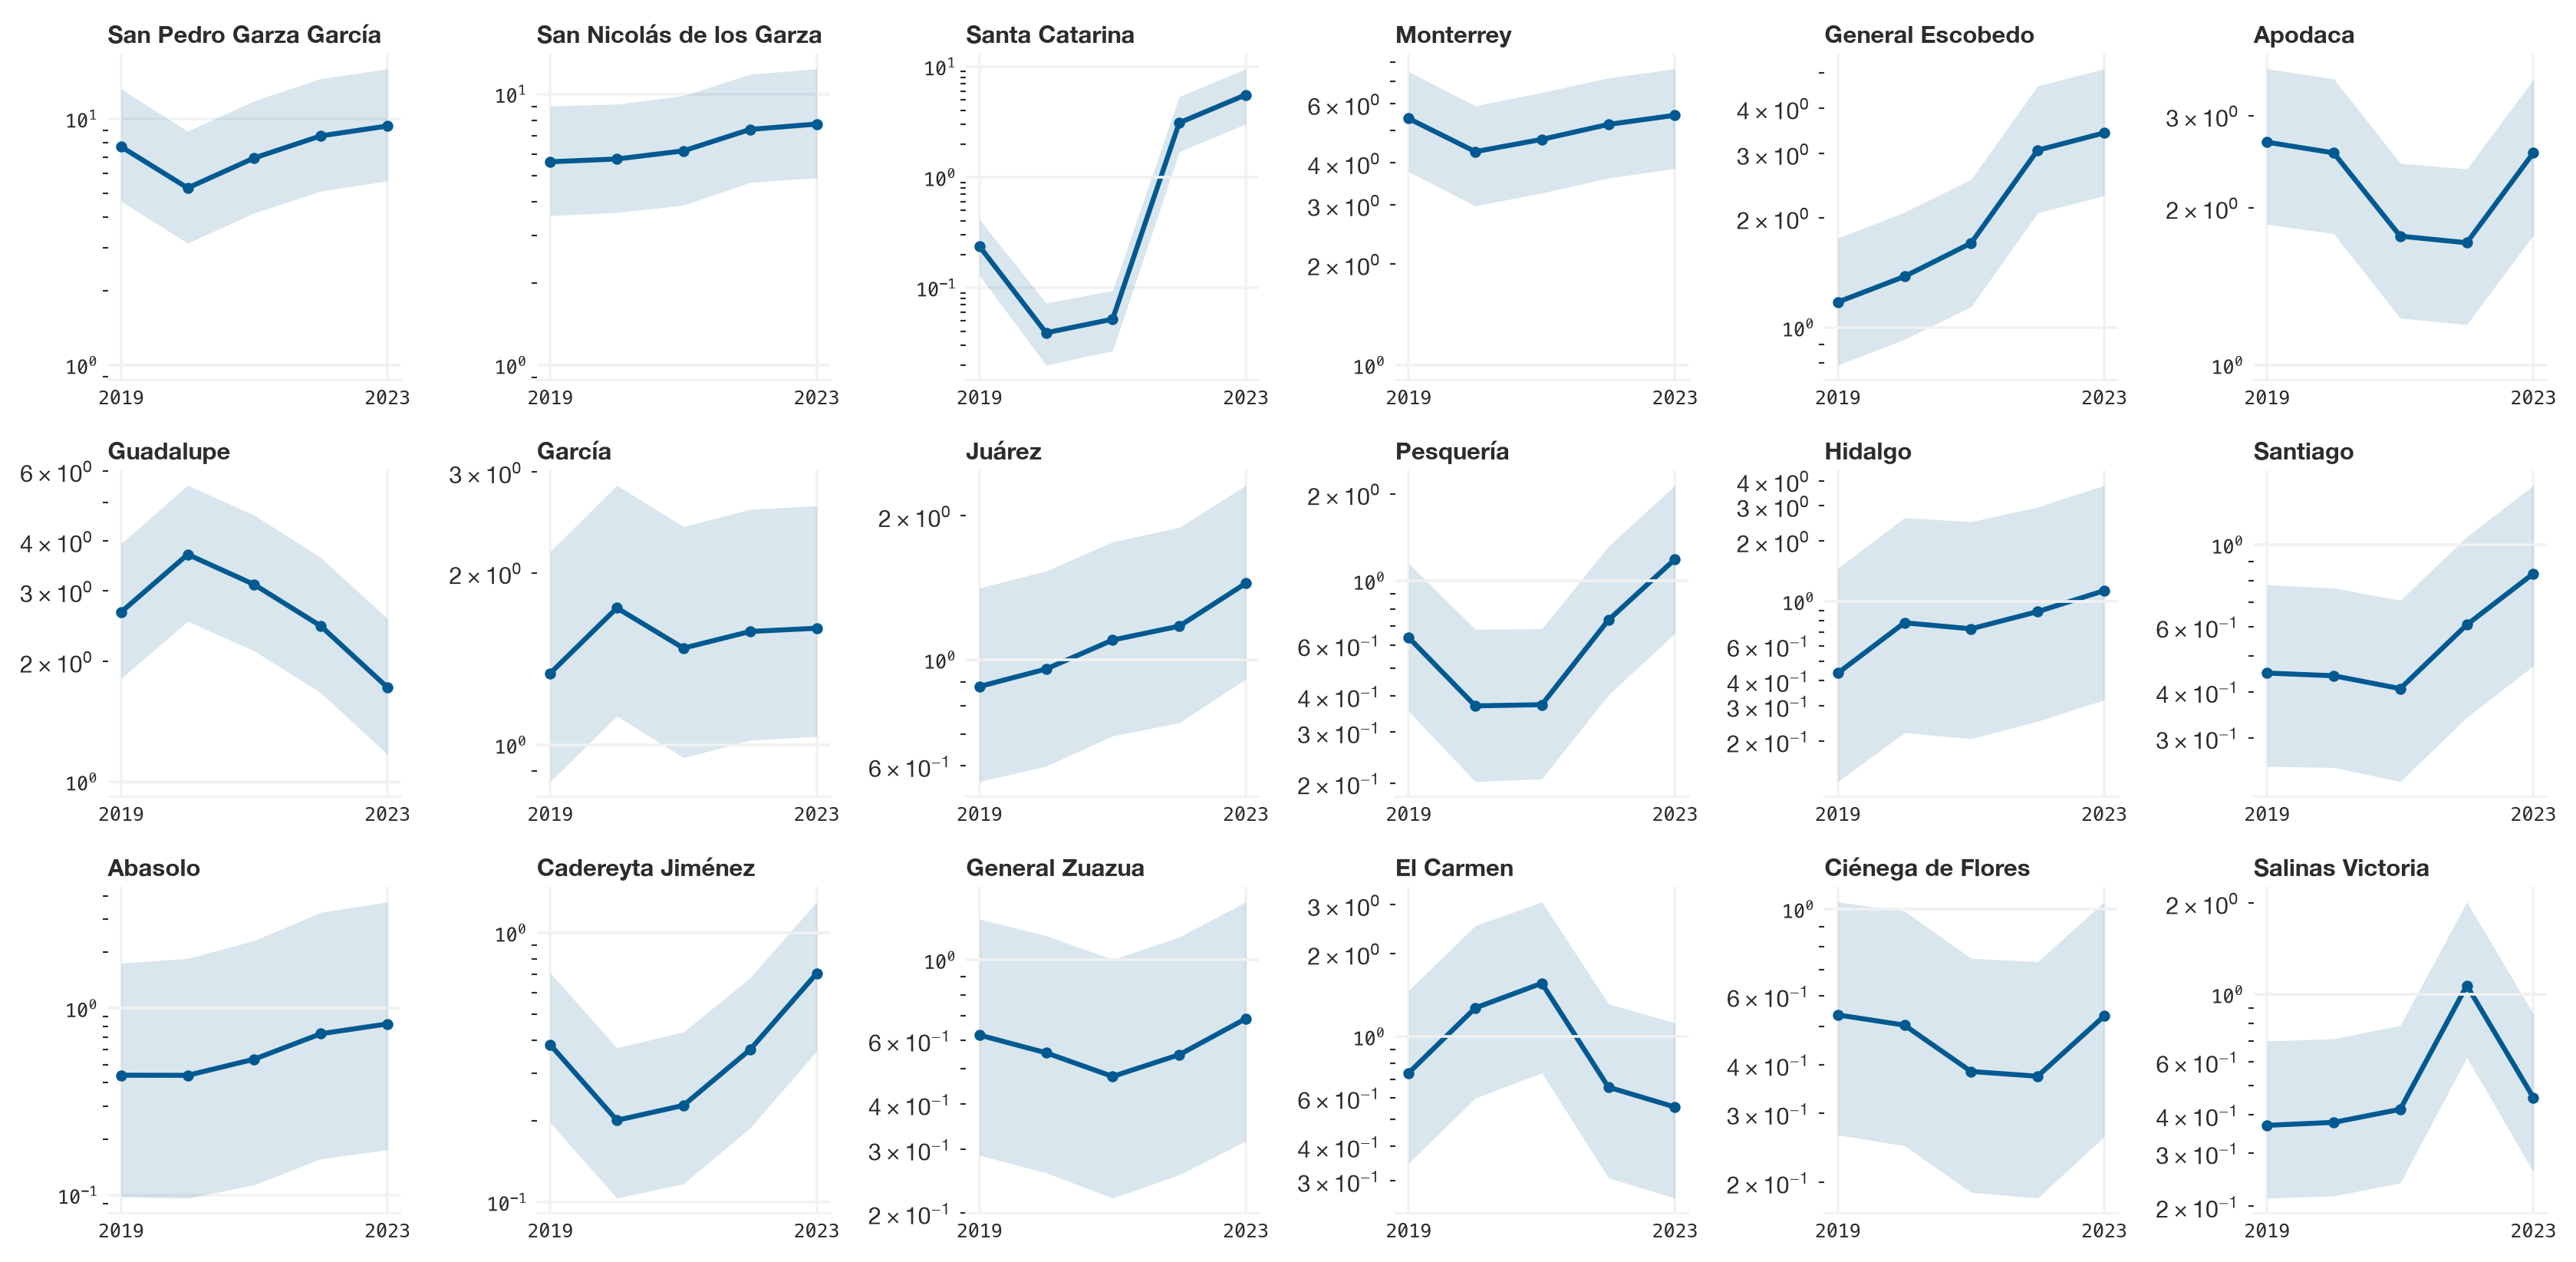
\includegraphics[width=\textwidth]{trayectorias}
\caption{Efecto municipal $e^{m_{j,a}}$ a posteriori, 2019--2023: mediana e
intervalo del 90\,\%, en escala logarítmica. Cada panel es un régimen de
reporte.}
\label{fig:res-trayectorias}
\end{figure*}

\paragraph{Perfil espacial neto del municipio.}
El efecto $u_i$ mide cuánto más o menos riesgo tiene cada celda que el
promedio de su municipio, estimado con la información de la celda y la de
sus vecinas (figura~\ref{fig:res-perfil}). Es el primer mapa del proyecto que
no depende de cuánto reporta cada municipio: cada celda se compara con su
propio municipio. Los corredores viales principales aparecen con $u_i > 0$, y
las colonias interiores y los bordes de la mancha urbana, con $u_i < 0$.

\begin{figure}
\centering
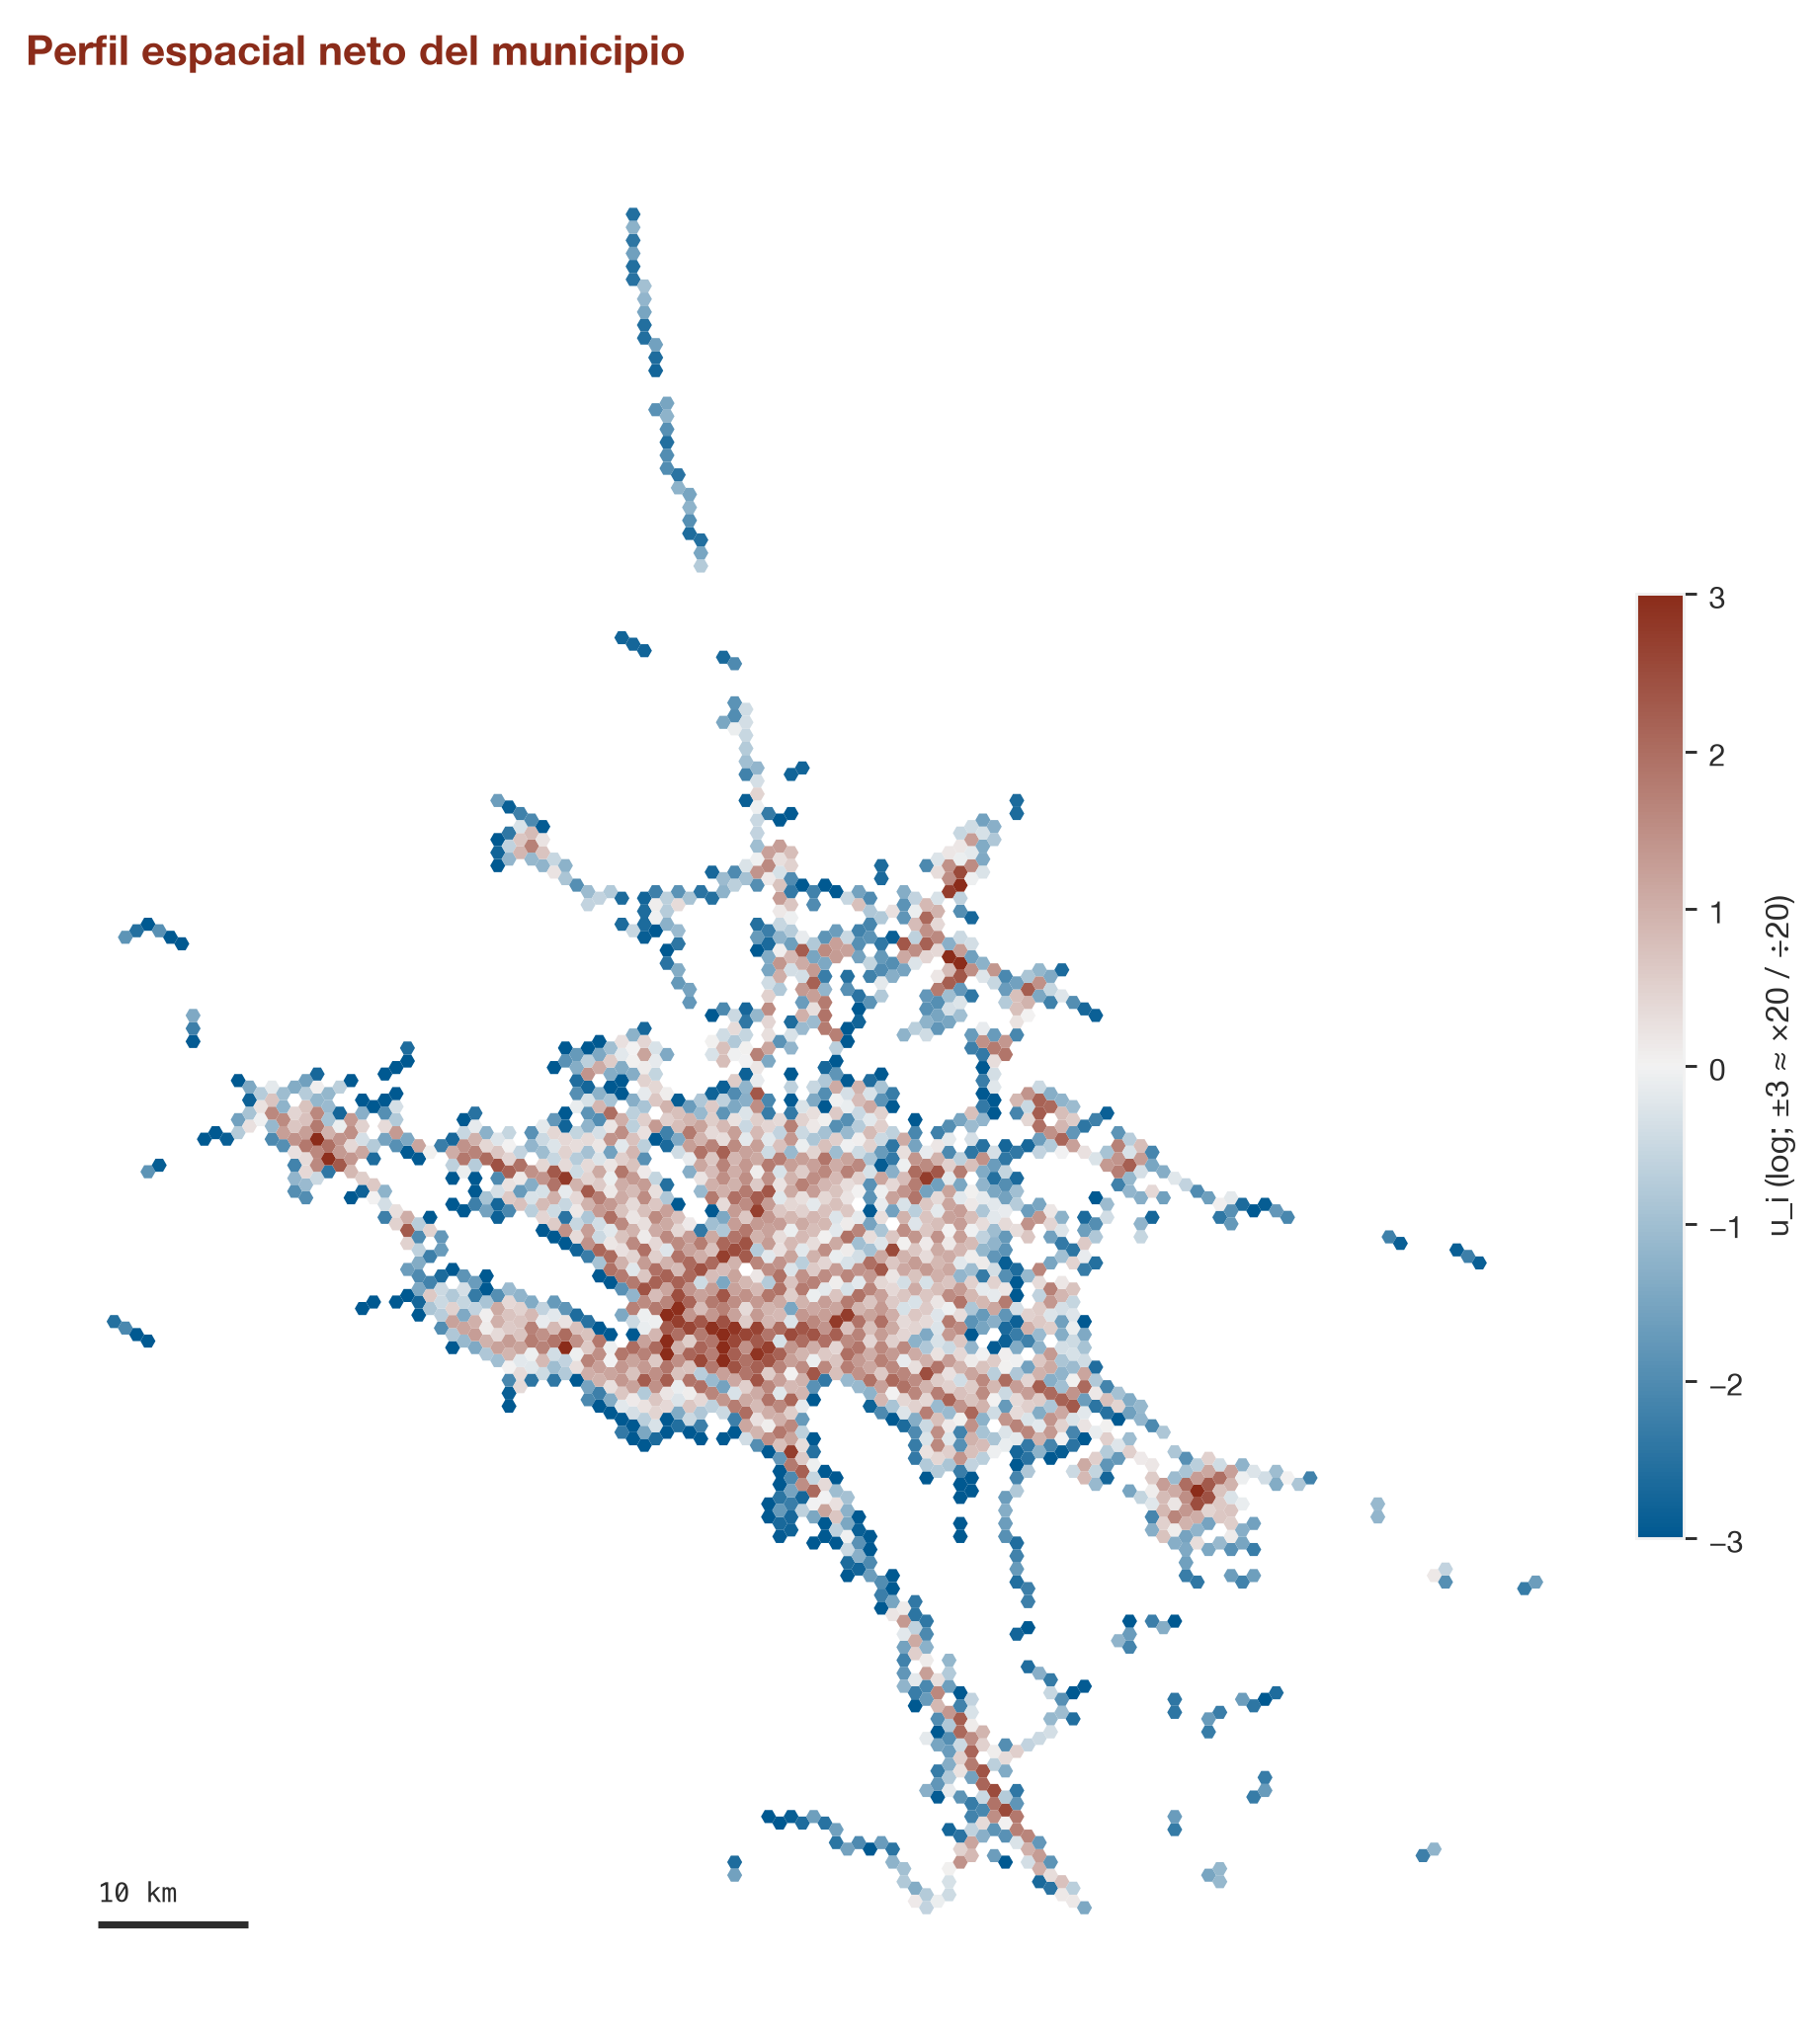
\includegraphics[width=\columnwidth]{perfil_u}
\caption{Mediana a posteriori de $u_i$, riesgo relativo de cada celda
respecto a su municipio (escala log; $\pm 3$ equivale a un factor de
$\approx 20$).}
\label{fig:res-perfil}
\end{figure}

En las 618 celdas con cinco accidentes o menos en cinco años, el modelo
encoge poco la estimación puntual respecto al estimador ingenuo (12\,\%),
pero su incertidumbre es el triple que la de las celdas con más de cien
accidentes (desviación posterior de 0,75 contra 0,25 en escala log;
figura~\ref{fig:res-shrinkage}). Dos celdas con el mismo $u_i$ y distinta
incertidumbre no justifican la misma intervención.

\begin{figure}
\centering
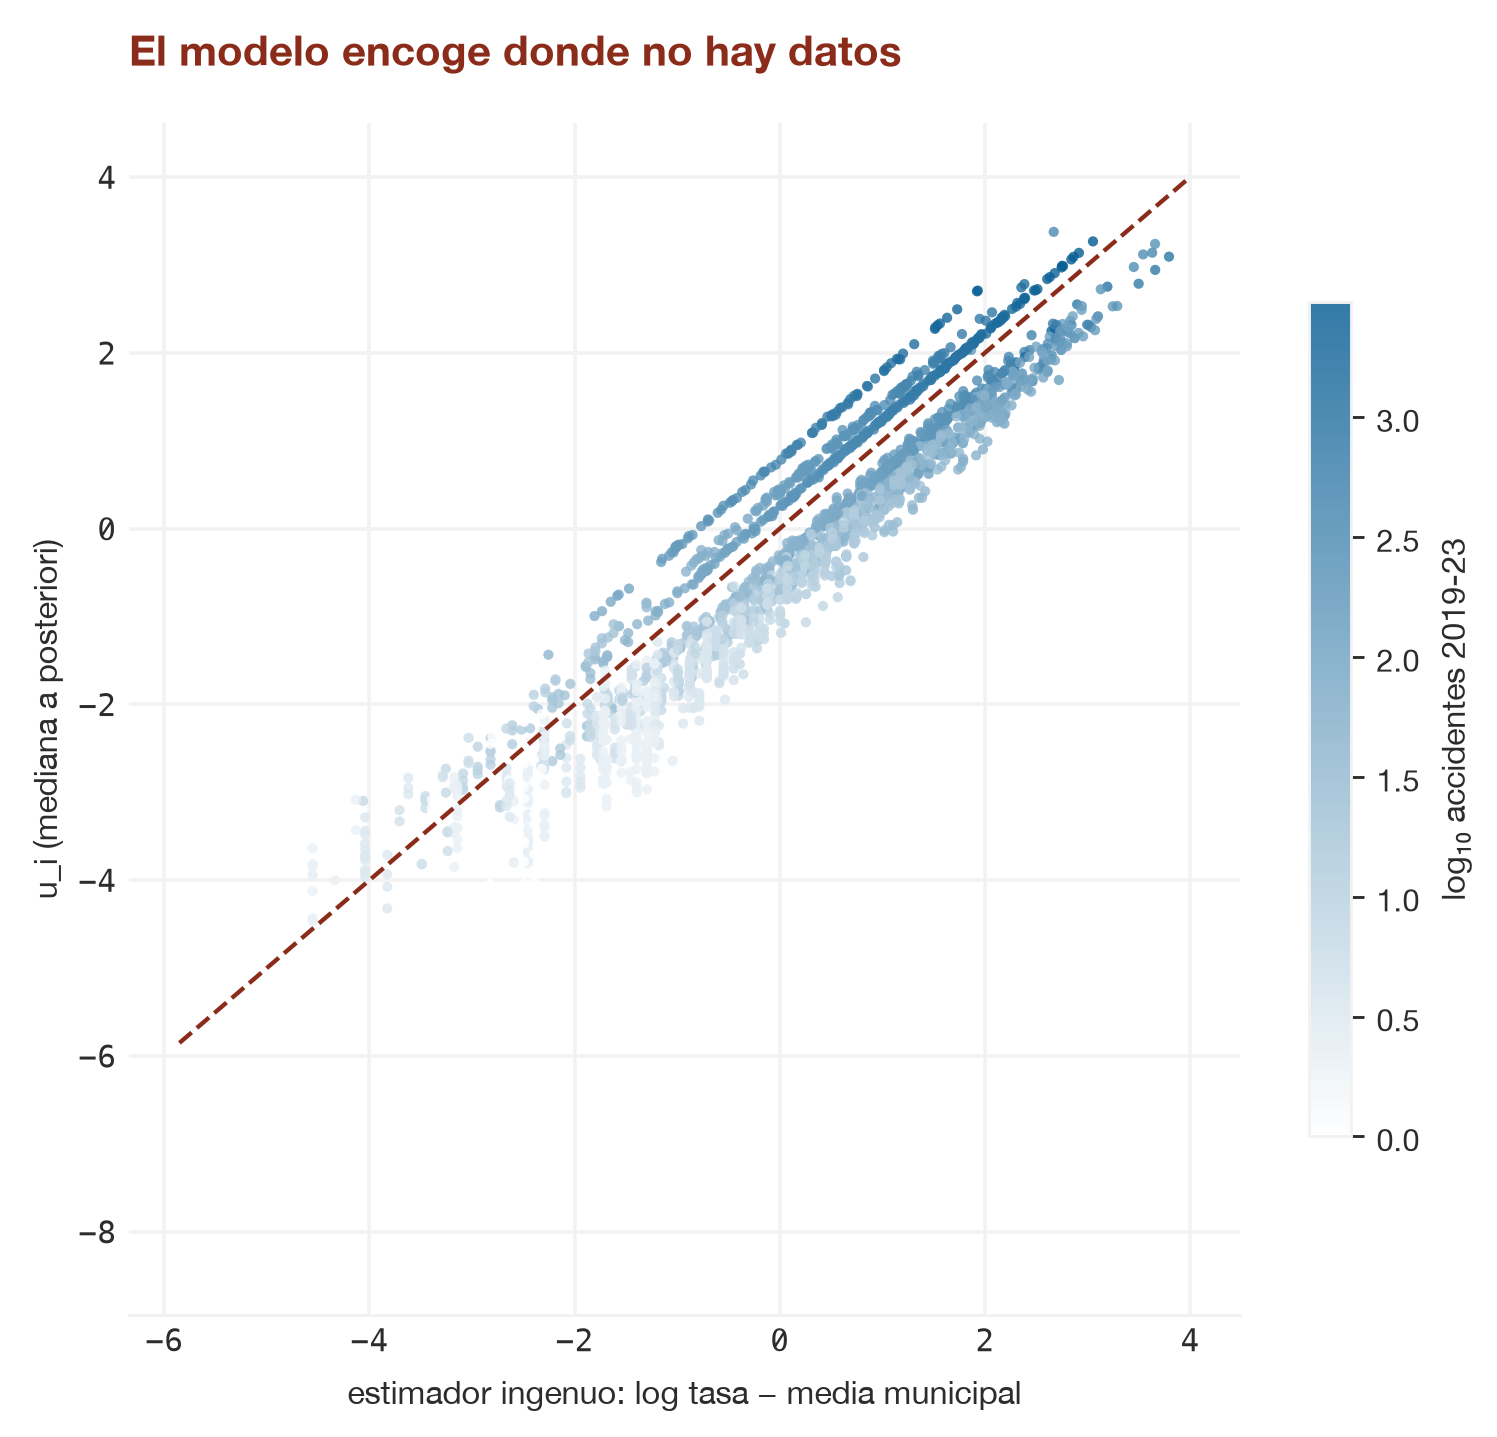
\includegraphics[width=0.9\columnwidth]{shrinkage}
\caption{Estimador ingenuo (log tasa menos media municipal) contra la
mediana a posteriori de $u_i$. El color indica los accidentes de cada celda
en entrenamiento; las celdas con pocos datos se encogen hacia su municipio y
sus vecinas.}
\label{fig:res-shrinkage}
\end{figure}

% ---------------------------------------------------------------------------
\subsection{Validación en 2024}\label{sec:res-validacion}
% ---------------------------------------------------------------------------

El pronóstico del modelo jerárquico se obtiene por simulación: para cada
muestra posterior se toma el nivel municipal de 2023, se combina con $u_i$ y
se simula un conteo Binomial Negativo. Es, por tanto, un pronóstico por
persistencia del régimen municipal (§\ref{sec:met-validacion}). Los
\emph{baselines} se recalculan a escala celda$\times$año para que la
comparación sea directa (cuadro~\ref{tab:res-validacion}).

\begin{table}
\centering\small
\caption{Validación en 2024 a escala celda$\times$año. M6 es el modelo
jerárquico con CAR y efecto municipal.}
\label{tab:res-validacion}
\begin{tabular}{@{}lrrrr@{}}
\toprule
Modelo & MAE & CRPS & Cob.\ 90\,\% & PAI \\
\midrule
M0  & 9,59 & 8,04 & 63\,\% & 8,41 \\
M0r & 8,15 & 6,56 & 68\,\% & 8,38 \\
M4  & 8,18 & 6,93 & \textbf{90\,\%} & 8,38 \\
\textbf{M6} & 8,19 & \textbf{6,17} & 87\,\% & 8,42 \\
\bottomrule
\end{tabular}
\end{table}

\begin{itemize}
\item \textbf{Calibración del total.} El jerárquico predice 70\,815
  accidentes para 2024 contra 71\,249 observados: un error del 0,6\,\%.
\item \textbf{Media.} Empata con M0r en MAE (8,19 contra 8,15). Lo
  predecible de 2024 es el nivel reciente de cada municipio por el perfil
  estable de cada celda, y un promedio bien elegido ya captura esa media.
\item \textbf{Distribución.} Mejora el CRPS \citep{gneiting_raftery_2007} del
  mejor \emph{baseline} en un 6\,\% (6,17 contra 6,56). El intervalo del
  90\,\% de M0r cubre solo el 68\,\% de las celdas, porque supone un Poisson
  sin sobredispersión ni régimen; el del jerárquico cubre el 87\,\%, cerca de
  su nivel nominal, aun sin incorporar el riesgo de cambio de régimen. M4
  cubre el 90\,\% a costa de un CRPS peor (6,93): sus intervalos son más
  anchos de lo necesario.
\item \textbf{Selección de zonas.} El PAI al 5\,\% es 8,42, prácticamente el
  mismo que el del histórico. El \emph{shrinkage} reordena la cola de la
  distribución de celdas, no la cabeza, que es donde se decide la selección.
\end{itemize}

Dos variantes se evaluaron y descartaron. La primera pronosticaba 2024 con
una innovación $t_3$ adicional en el nivel municipal; como
$\E[e^{T}] = \infty$ para cualquier $t$ de Student, la media predictiva no
existe, y numéricamente la suma de medias dio 2,3 millones de accidentes
contra 71 mil observados, con valores que cambiaban con la semilla. La
segunda añadía una deriva por municipio para capturar el crecimiento
periférico: la posterior la encogió a cero ($\sigma_d = 0{,}07$), produjo 46
divergencias y no mejoró el CRPS. Con cinco años y saltos de régimen, los
datos no distinguen una tendencia de una racha de innovaciones.

En síntesis, el PAI al 5\,\% se mantuvo en 8,4 en todos los modelos, desde el
conteo histórico hasta el jerárquico: el \emph{dónde} lo determina el
historial de cada celda. Lo que el modelo jerárquico añade es una
distribución predictiva calibrada y un perfil espacial neto del régimen de
reporte municipal.
